\documentclass[9pt,pdftex,aspectratio=1610]{beamer}
\usepackage{amsmath, amsthm, amssymb}
\usepackage{color}
\usepackage{subfigure}
\usepackage{hyperref}
\usepackage{tabularx}
\usepackage{ragged2e}
\usepackage{booktabs}
\usepackage{multirow}
\usepackage{natbib}
\usecolortheme{dolphin}
\linespread{1.3}
\definecolor{nblue}{RGB}{0,0,128}
\bibliographystyle{ecta}
\setbeamercovered{transparent}


\newcolumntype{Y}{>{\RaggedRight\arraybackslash}X}
%\setbeamerfont{alerted text}{series=\bfseries}

%\everymath{\displaystyle}

\hypersetup{colorlinks=true, linkcolor=nblue,
citecolor=nblue, urlcolor=nblue, bookmarks=false,
pdfpagemode=UseNone,
pdfstartview={XYZ null null 1.25},
pdftitle={The Welfare Effects of Encouraging Rural-Urban Migration},
pdfauthor={David Lagakos, Mushfiq Mobarak, Michael E. Waugh},
pdfkeywords={economics,macroeconomics,development economics,migration,selection,spatial misallocation,welfare,Roy model,urban-rural wage gaps,agricultural productivity gaps,productivity},
}


\setbeamertemplate{navigation symbols}{}
\setbeamertemplate{footline}[frame number]
\setbeamertemplate{theorems}[numbered]
\setbeamertemplate{itemize subitem}[circle]
\setbeamertemplate{enumerate items}[default]

\setbeamerfont{frametitle}{size= \large}
\setbeamerfont{ framesubtitle }{size = \footnotesize}
\setbeamertemplate{frametitle}
{
\medskip
\smallskip
{\textsf{\underline{\insertframetitle\phantom{))))))))}}}}}
\setbeamertemplate{items}[circle]
\setbeamertemplate{itemize subitem}[circle]

\theoremstyle{definition}


\newtheorem{as}{Assumption}
\newtheorem{df}{Definition}
\newtheorem{lm}{Lemma}
\newtheorem{pf}{Proposition}

\usepackage[normalem]{ulem}
\newcommand\redout{\bgroup\markoverwith
{\textcolor{red}{\rule[.5ex]{1pt}{1pt}}}\ULon}

%%%%%%%%%%%%%%%%%%%%%%%%%%%%%%%%%%%%%%%%%%%%%%%%%%%%%%%%%%%%%%%%%%%%%%%%%%%%%%%%%%%%%%%%%%%%%%%%%
%%%%%%%%%%%%%%%%%%%%%%%%%%%%%%%%%%%%%%%%%%%%%%%%%%%%%%%%%%%%%%%%%%%%%%%%%%%%%%%%%%%%%%%%%%%%%%%%%

\title{\Large The Welfare Effects of Encouraging Rural-Urban Migration}
\institute[Foo and Bar]{\normalsize\begin{tabular}[h]{ccc}
David Lagakos & A. Mushfiq Mobarak &  Michael E. Waugh  \\
Boston University and NBER & Yale University and NBER & FRB Minneapolis and NBER\\
\end{tabular}}

\date{\today}


\begin{document}


\begin{frame}
\titlepage
\setcounter{framenumber}{0}
\section{}
\end{frame}

%%%%%%%%%%%%%%%%%%%%%%%%%%%%%%%%%%%%%%%%%%%%%%%%%%%%%%%%%%%%%%%%%%%%%%%%%%%%%%%%%%%%%%%%%%%%%%%%%
%%%%%%%%%%%%%%%%%%%%%%%%%%%%%%%%%%%%%%%%%%%%%%%%%%%%%%%%%%%%%%%%%%%%%%%%%%%%%%%%%%%%%%%%%%%%%%%%%

\begin{frame}[t]
\frametitle{The Context: The Migration Experiment in Rural Bangladesh}
The Migration experiment of \citet*{brch14}
\begin{itemize}
\smallskip
\item 100 randomly selected villages in the Rangpur region of Bangladesh. Selected 19 households in each village.
\smallskip
\item Villages randomly put into four groups: cash, credit, information, control.
\smallskip
\end{itemize}
\bigskip
Households in the cash group given 600 Taka (\$8.50) conditional on migration. Given 200 Taka if they reported in at the destination. What happened? \\
\begin{itemize}
\smallskip
\item 22\% increase in migration in treatment relative to control (58\% vs 36\%).
\smallskip
\item 9\% increase in migration in the subsequent year.
\smallskip
\item Migrants increased consumption by 10\%, OLS.
\smallskip
\item \emph{Induced} migrants increased their consumption by 30\% relative to the average household. Also known as the ``LATE''.
\end{itemize}
\end{frame}

%%%%%%%%%%%%%%%%%%%%%%%%%%%%%%%%%%%%%%%%%%%%%%%%%%%%%%%%%%%%%%%%%%%%%%%%%%%%%%%%%%%%%%%%%%%%%%%%%
%%%%%%%%%%%%%%%%%%%%%%%%%%%%%%%%%%%%%%%%%%%%%%%%%%%%%%%%%%%%%%%%%%%%%%%%%%%%%%%%%%%%%%%%%%%%%%%%%

\begin{frame}[t]{What We Do\ldots}
Build a spatial incomplete markets model, discipline it using the experiment, then ask questions:\\
\bigskip
\textbf{1.} What happened in the experiment?
\begin{itemize}
\smallskip
\item In bad states of the world, urban migration is relatively more beneficial $\Rightarrow$ migration is insurance.
\smallskip
\item And negative selection (LATE $>$ OLS) in the data reveals this.
\end{itemize}
\bigskip
\textbf{2.} What are the welfare gains from conditional migration subsidies? \\
\begin{itemize}
\smallskip
\item Gains because they target those who need transfers the most, even if tax financed.
\smallskip
\end{itemize}
\bigskip
\textbf{3.} What is the socially optimal outcome? \\
\begin{itemize}
\smallskip
\item Directly provide insurance with \textcolor{red}{\textbf{less}} movement of households across locations.
\smallskip
\end{itemize}
\end{frame}


%%%%%%%%%%%%%%%%%%%%%%%%%%%%%%%%%%%%%%%%%%%%%%%%%%%%%%%%%%%%%%%%%%%%%%%%%%%%%%%%%%%%%%%%%%%%%%%%%
%%%%%%%%%%%%%%%%%%%%%%%%%%%%%%%%%%%%%%%%%%%%%%%%%%%%%%%%%%%%%%%%%%%%%%%%%%%%%%%%%%%%%%%%%%%%%%%%%

\begin{frame}
\vspace{1cm}
\begin{center}
\textbf{\textcolor{blue}{\large Model}}
\end{center}
\end{frame}

%%%%%%%%%%%%%%%%%%%%%%%%%%%%%%%%%%%%%%%%%%%%%%%%%%%%%%%%%%%%%%%%%%%%%%%%%%%%%%%%%%%%%%%%%%%%%%%%%
%%%%%%%%%%%%%%%%%%%%%%%%%%%%%%%%%%%%%%%%%%%%%%%%%%%%%%%%%%%%%%%%%%%%%%%%%%%%%%%%%%%%%%%%%%%%%%%%%

\begin{frame}[t]{Model: Households and Preferences}
\medskip
Unit mass of households; preferences:
\begin{align*}
\sum_{t = 0}^{\infty} \beta^t u(c_t) \bar u^{x_t}
\end{align*}\\
\medskip
\begin{itemize}
\item $\bar u$ is disutility of migration
\smallskip
\item $x_t \in \{0,1\}$, takes on value 1 iff household is ``inexperienced at migration'' and in the urban area.
\smallskip
\smallskip
\item $u(c_t) = \frac{c_t^{1-\alpha}}{1-\alpha}$
\end{itemize}
\bigskip
Also face additive taste shocks across moving options, which are iid across time and options and drawn from a Type-1 EV distribution with scale parameter $\sigma_{\nu}$
\end{frame}

%%%%%%%%%%%%%%%%%%%%%%%%%%%%%%%%%%%%%%%%%%%%%%%%%%%%%%%%%%%%%%%%%%%%%%%%%%%%%%%%%%%%%%%%%%%%%%%%%
%%%%%%%%%%%%%%%%%%%%%%%%%%%%%%%%%%%%%%%%%%%%%%%%%%%%%%%%%%%%%%%%%%%%%%%%%%%%%%%%%%%%%%%%%%%%%%%%%

\begin{frame}[t]{Model: Experience}
A household is either ``experienced'' or ``inexperienced'' at migration.\\
\medskip
Experience is acquired by being in the urban area, is lost by being away\ldots\\
\bigskip
After each period in the \underline{urban} area,
\begin{itemize}
\item Inexperienced households remain so with probability $\lambda$, and become experienced with probability $1-\lambda$,
\smallskip
\item Experienced households stay experienced.
\end{itemize}
\bigskip
After each period in the \underline{rural} area,
\begin{itemize}
\item Experienced households stay experienced with probability $\pi$ and loose experience with probability $1-\pi$,
\smallskip
\item Inexperienced households stay inexperienced.
\end{itemize}
\end{frame}


%%%%%%%%%%%%%%%%%%%%%%%%%%%%%%%%%%%%%%%%%%%%%%%%%%%%%%%%%%%%%%%%%%%%%%%%%%%%%%%%%%%%%%%%%%%%%%%%%
%%%%%%%%%%%%%%%%%%%%%%%%%%%%%%%%%%%%%%%%%%%%%%%%%%%%%%%%%%%%%%%%%%%%%%%%%%%%%%%%%%%%%%%%%%%%%%%%%

\begin{frame}[t]{Model: Production Technologies and Seasons}
One homogenous good produced in both locations and competitive markets.
\medskip
Production technology in rural area:
\begin{align*}
Y_r = A_{ri} N_r^{\phi}
\end{align*}\\
where $0<\phi<1$; $A_{ri}$ is rural productivity indexed by season $i$, with $A_{rg} > A_{rl}$ \\
\begin{itemize}
\smallskip
\item Deterministic transition: If rural productivity is $A_{rg}$, then the economy transits to $A_{rl}$ next period.
\smallskip
\item Idea: mimic seasonal agricultural crop cycles
\smallskip
\end{itemize}
\medskip
Production technology in urban area
\begin{align*}
Y_u = A_u N_u
\end{align*}
\end{frame}

%%%%%%%%%%%%%%%%%%%%%%%%%%%%%%%%%%%%%%%%%%%%%%%%%%%%%%%%%%%%%%%%%%%%%%%%%%%%%%%%%%%%%%%%%%%%%%%%%
%%%%%%%%%%%%%%%%%%%%%%%%%%%%%%%%%%%%%%%%%%%%%%%%%%%%%%%%%%%%%%%%%%%%%%%%%%%%%%%%%%%%%%%%%%%%%%%%%

\begin{frame}[t]{Model: Household Location-Specific Productivity}
Each household has permanent productivity types as in Roy (1951)
\begin{itemize}
\smallskip
\item $z$ permanent productivity in urban area. $z \sim$ Pareto($\theta$).
\smallskip
\item no permanent productivity differences in the rural area.
\end{itemize}
\bigskip
Each household experiences transitory shocks $s$ that follows an AR(1) process
\begin{align*}
\log s_{t+1} = \rho \log s_{t} + \epsilon_{t+1} \ \ \  \mbox{with} \ \  \ \epsilon_{t+1} \sim \mathcal{N}(0,\sigma_{s}).
\end{align*}\\
\bigskip
Household-specific efficiency units of labor in each location:
\begin{itemize}
\smallskip
\item $s$ in the rural area.
\smallskip
\item $zs^\gamma$ in the urban area.
\smallskip
\item $\gamma$ is affecting relative returns and volatility to locating in different areas.
\end{itemize}
\end{frame}

%%%%%%%%%%%%%%%%%%%%%%%%%%%%%%%%%%%%%%%%%%%%%%%%%%%%%%%%%%%%%%%%%%%%%%%%%%%%%%%%%%%%%%%%%%%%%%%%%
%%%%%%%%%%%%%%%%%%%%%%%%%%%%%%%%%%%%%%%%%%%%%%%%%%%%%%%%%%%%%%%%%%%%%%%%%%%%%%%%%%%%%%%%%%%%%%%%%

\begin{frame}[t]{Model: Options}
Households in the rural area can\ldots
\begin{itemize}
\smallskip
\item[1.] Work in the rural area.
\smallskip
\item[2.] Pay fixed cost $m_T$, work in the urban area the next period, return to rural.\\ \smallskip This is \underline{seasonal migration}.
\smallskip
\item[3.] Pay fixed cost $m_p > m_T$, move to urban area next period, stay indefinitely.\\ \smallskip This is \underline{permanent migration}.
\end{itemize}
\bigskip
Households in the urban area can\ldots
\begin{itemize}
\smallskip
\item[1.]  Work in the urban area.
\smallskip
\item[2.]  Pay fixed cost $m_p$, work in rural area for the indefinite future.
\end{itemize}
\end{frame}

%%%%%%%%%%%%%%%%%%%%%%%%%%%%%%%%%%%%%%%%%%%%%%%%%%%%%%%%%%%%%%%%%%%%%%%%%%%%%%%%%%%%%%%%%%%%%%%%%
%%%%%%%%%%%%%%%%%%%%%%%%%%%%%%%%%%%%%%%%%%%%%%%%%%%%%%%%%%%%%%%%%%%%%%%%%%%%%%%%%%%%%%%%%%%%%%%%%

\begin{frame}[t]{Model: Asset Choices}
Households can accumulate a non-state contingent asset, $a$, with gross rate of return, $R$. Assets move with the household.
\begin{itemize}
\smallskip
\item Asset holdings can not be negative (no borrowing).
\smallskip
\item $R$ is exogenous (small open economy).
\end{itemize}
\end{frame}

%%%%%%%%%%%%%%%%%%%%%%%%%%%%%%%%%%%%%%%%%%%%%%%%%%%%%%%%%%%%%%%%%%%%%%%%%%%%%%%%%%%%%%%%%%%%%%%%%
%%%%%%%%%%%%%%%%%%%%%%%%%%%%%%%%%%%%%%%%%%%%%%%%%%%%%%%%%%%%%%%%%%%%%%%%%%%%%%%%%%%%%%%%%%%%%%%%%

\begin{frame}[t]{Who moves? When do they move?}
All else equal, seasonal migration more likely:
\begin{itemize}
\smallskip
\item In the lean season,
\smallskip
\item Among agents with higher $z$,
\smallskip
\item When experienced.
\end{itemize}
\bigskip
The open question is how migration depends upon:
\begin{itemize}
\smallskip
\item The transitory shock, $s$
\smallskip
\item Asset holdings, $a$.
\end{itemize}
\bigskip
Model flexible; experimental data disciplines whether e.g. agents migrate when transitory shock and assets are sufficiently high or sufficiently low.
\end{frame}

%%%%%%%%%%%%%%%%%%%%%%%%%%%%%%%%%%%%%%%%%%%%%%%%%%%%%%%%%%%%%%%%%%%%%%%%%%%%%%%%%%%%%%%%%%%%%%%%%
%%%%%%%%%%%%%%%%%%%%%%%%%%%%%%%%%%%%%%%%%%%%%%%%%%%%%%%%%%%%%%%%%%%%%%%%%%%%%%%%%%%%%%%%%%%%%%%%%

\begin{frame}
\vspace{1cm}
\begin{center}
\textbf{\textcolor{blue}{\large Calibration}}
\end{center}
\end{frame}

%%%%%%%%%%%%%%%%%%%%%%%%%%%%%%%%%%%%%%%%%%%%%%%%%%%%%%%%%%%%%%%%%%%%%%%%%%%%%%%%%%%%%%%%%%%%%%%%%
%%%%%%%%%%%%%%%%%%%%%%%%%%%%%%%%%%%%%%%%%%%%%%%%%%%%%%%%%%%%%%%%%%%%%%%%%%%%%%%%%%%%%%%%%%%%%%%%%

\begin{frame}[t]{Calibration Overview}
Parameterize productivity distribution \& shocks, pre-assign some values \\
\bigskip
Remaining parameters picked to minimize distance between model \& data
\begin{itemize}
\smallskip
\item[1.] Experimental moments: Perform the \citet{brch14} experiment in model.
\smallskip
\item[2.] Cross-sectional moments: urban-rural wage gap, rural share, variances of consumption and earnings.
\end{itemize}
\bigskip
\end{frame}

%%%%%%%%%%%%%%%%%%%%%%%%%%%%%%%%%%%%%%%%%%%%%%%%%%%%%%%%%%%%%%%%%%%%%%%%%%%%%%%%%%%%%%%%%%%%%%%%
%%%%%%%%%%%%%%%%%%%%%%%%%%%%%%%%%%%%%%%%%%%%%%%%%%%%%%%%%%%%%%%%%%%%%%%%%%%%%%%%%%%%%%%%%%%%%%%%

\begin{frame}[t]{Pre-Assigned Parameters}
\begin{table}[!t]
\refstepcounter{table}
\footnotesize
\setlength {\tabcolsep}{1.25mm}
\renewcommand{\arraystretch}{1.75}
\begin{center}
\begin{tabular}{l l l }
\multicolumn{3}{c}{\textbf{\small Pre-Assigned Parameters}}\\
\hline
\hline
Parameter & Value & Source \\
\hline
Time period & Half year  & --- \\
Risk aversion, $\alpha$  & 2.0 & --- \\
Discount factor, $\beta$ & 0.95 & ---  \\
Gross real interest rate, $R$ & 0.95 & 1/ gross inflation rate \\
Rural seasonal productivity, $A_{rl}/A_{rg}$ & 50\% drop in rural inc. & --- \\
Returns to Scale in Rural P.F. & $\phi$ & AKM (2018) experiment\\
Seasonal moving costs, $m_T$ &  10\% of rural consumption & Bryan et al. (2014) \\
Permanent moving costs, $m_p$  &  $2 \times m_T$ & -- \\
\hline
\end{tabular}
\end{center}
\end{table}
\end{frame}

%%%%%%%%%%%%%%%%%%%%%%%%%%%%%%%%%%%%%%%%%%%%%%%%%%%%%%%%%%%%%%%%%%%%%%%%%%%%%%%%%%%%%%%%%%%%%%%%%%
%%%%%%%%%%%%%%%%%%%%%%%%%%%%%%%%%%%%%%%%%%%%%%%%%%%%%%%%%%%%%%%%%%%%%%%%%%%%%%%%%%%%%%%%%%%%%%%%%%

\begin{frame}[t]{Parameters to Calibrate}
\begin{itemize}
\item Productivity urban area: $A_u$
\smallskip
\item Shape parameter, urban permanent productivity: $\theta$
\smallskip
\item Standard deviation of transitory shocks: $\sigma_s$
\smallskip
\item Urban relative risk parameter: $\gamma$
\smallskip
\item Persistence of transitory shocks: $\rho$
\smallskip
\item Disutility of migration: $\bar u$
\smallskip
\item Probability of gaining experience: $1-\lambda$
\smallskip
\item Probability of losing experience: $1-\pi$
\smallskip
\item Additive Type-1 EV taste shocks: $\sigma_{\nu}$
\end{itemize}
\medskip
plus two sources of measurement error\ldots to match 11 moments.
\end{frame}

%%%%%%%%%%%%%%%%%%%%%%%%%%%%%%%%%%%%%%%%%%%%%%%%%%%%%%%%%%%%%%%%%%%%%%%%%%%%%%%%%%%%%%%%%%%%%%%%%
%%%%%%%%%%%%%%%%%%%%%%%%%%%%%%%%%%%%%%%%%%%%%%%%%%%%%%%%%%%%%%%%%%%%%%%%%%%%%%%%%%%%%%%%%%%%%%%%%

\begin{frame}[t]{Calibration: The BCM (2014) Field Experiment}
The BCM (2014) field experiment results / our calibration targets:
\begin{itemize}
\smallskip
\item 22\% increase in migration in treatment relative to control (58\% vs 36\%).
\smallskip
\item 9\% increase in migration in the subsequent year.
\smallskip
\item Migrants increased consumption by 10\%, OLS.
\smallskip
\item \emph{Induced} migrants increased their consumption by 30\% relative to the average household. Also known as the ``LATE''.
\end{itemize}
\end{frame}

%%%%%%%%%%%%%%%%%%%%%%%%%%%%%%%%%%%%%%%%%%%%%%%%%%%%%%%%%%%%%%%%%%%%%%%%%%%%%%%%%%%%%%%%%%%%%%%%%
%%%%%%%%%%%%%%%%%%%%%%%%%%%%%%%%%%%%%%%%%%%%%%%%%%%%%%%%%%%%%%%%%%%%%%%%%%%%%%%%%%%%%%%%%%%%%%%%%

\begin{frame}[t]{Calibration: Performing the BCM (2014) Experiment in the Model}
\textbf{1.} Solve for optimal policies of households when offered $m_T$, if they move.
\begin{itemize}
\smallskip
\item Offer is one-time, unanticipated, no general equilibrium effects.
\end{itemize}
\bigskip
\textbf{2.} Randomly sample rural households in the stationary distribution consistent with BCM (2014) sample selection\ldots
\begin{itemize}
\smallskip
\item Offer households $m_T$, and follow.
\smallskip
\item Compare with the actions of the same households absent the offer.
\end{itemize}
\bigskip
\textbf{3.} Compute statistics in the model as done with the data.
\end{frame}

%%%%%%%%%%%%%%%%%%%%%%%%%%%%%%%%%%%%%%%%%%%%%%%%%%%%%%%%%%%%%%%%%%%%%%%%%%%%%%%%%%%%%%%%%%%%%%%%%
%%%%%%%%%%%%%%%%%%%%%%%%%%%%%%%%%%%%%%%%%%%%%%%%%%%%%%%%%%%%%%%%%%%%%%%%%%%%%%%%%%%%%%%%%%%%%%%%%

\begin{frame}[t]{Calibration Results | Model Fit}
\begin{table}[!t]
\footnotesize
\setlength {\tabcolsep}{2.95mm}
\renewcommand{\arraystretch}{1.}
\begin{center}
\begin{tabular}{l l c c}
\multicolumn{4}{c}{\textbf{\small Moments Targeted in the Estimation}}\\
\hline
\hline
Moments & Data & Model \\
\hline
Control: Variance of rural log consumption growth & $\begin{array}{c}0.19\vspace{-.15cm}\\ \scriptstyle (0.03)\end{array}$
& $\begin{array}{c}0.19\vspace{-.15cm}\\ \scriptstyle \phantom{(0.03)}\end{array}$\\

Control: Percent of rural households with no liquid assets &
$\begin{array}{c}47\vspace{-.15cm}\\ \scriptstyle (1.13)\end{array}$ &
$\begin{array}{c}48\vspace{-.15cm}\\ \scriptstyle \phantom{(1.13)}\end{array}$\\

Control: Seasonal migration rate &
$\begin{array}{c}36\vspace{-.15cm}\\ \scriptstyle (2.64)\end{array}$ &
$\begin{array}{c}36\vspace{-.15cm}\\ \scriptstyle \phantom{(2.64)}\end{array}$ &\\

 Control: Share of Repeat Migrants&
$\begin{array}{c}68\vspace{-.15cm}\\ \scriptstyle (0.46)\end{array}$ &
$\begin{array}{c}70\vspace{-.15cm}\\ \scriptstyle \phantom{(0.46)}\end{array}$ & \\

Control: Consumption increase of migrants (OLS) &
$\begin{array}{c}10\vspace{-.15cm}\\ \scriptstyle (4.47)\end{array}$ &
$\begin{array}{c}10\vspace{-.15cm}\\ \scriptstyle \phantom{(4.47)}\end{array}$ & \\


Treatment: Seasonal migration relative to control &
 $\begin{array}{c}22\vspace{-.15cm}\\ \scriptstyle (2.39)\end{array}$ &
$\begin{array}{c}21\vspace{-.15cm}\\ \scriptstyle \phantom{(2.39)}\end{array}$ & \\


Treatment: Seasonal migration relative to control in year 2 &
 $\begin{array}{c}9\vspace{-.15cm}\\ \scriptstyle (2.44)\end{array}$ &
$\begin{array}{c}4\vspace{-.15cm}\\ \scriptstyle \phantom{(2.44)}\end{array}$ & \\


Treatment: Consumption increase of induced migrants (LATE)  &
$\begin{array}{c}30\vspace{-.15cm}\\ \scriptstyle (9.67)\end{array}$ &
$\begin{array}{c}29\vspace{-.15cm}\\ \scriptstyle \phantom{(9.67)}\end{array}$ & \\

\hline
Urban-Rural wage gap &
$\begin{array}{c}1.89\vspace{-.15cm}\\ \scriptstyle (0.18)\end{array}$ &
$\begin{array}{c}1.89\vspace{-.15cm}\\ \scriptstyle \phantom{(0.18)}\end{array}$ & \\

Percent in rural area &
$\begin{array}{c}62\vspace{-.15cm}\\ \scriptstyle (1.36)\end{array}$ &
$\begin{array}{c}60\vspace{-.15cm}\\ \scriptstyle \phantom{(0.18)}\end{array}$ & \\

Variance of log urban wages  &
$\begin{array}{c}0.56\vspace{-.15cm}\\ \scriptstyle (0.06)\end{array}$ &
$\begin{array}{c}0.56\vspace{-.15cm}\\ \scriptstyle \phantom{(0.18)}\end{array}$ & \\
\hline
\end{tabular}
\parbox[c]{4.25in}{\vspace{.1cm}
{\footnotesize \textbf{Note:} The table reports the moments targeted using simulated method of moments, their values in the data and in the model, and the standard errors of the empirical moments.}
}
\end{center}
\end{table}
\end{frame}

%%%%%%%%%%%%%%%%%%%%%%%%%%%%%%%%%%%%%%%%%%%%%%%%%%%%%%%%%%%%%%%%%%%%%%%%%%%%%%%%%%%%%%%%%%%%%%%%%
%%%%%%%%%%%%%%%%%%%%%%%%%%%%%%%%%%%%%%%%%%%%%%%%%%%%%%%%%%%%%%%%%%%%%%%%%%%%%%%%%%%%%%%%%%%%%%%%%
\begin{frame}[t]{Calibration Results | Parameters }
\small
\begin{table}[!t]
\footnotesize
\refstepcounter{table}
\label{ta:cal}
\setlength {\tabcolsep}{4.5mm}
\renewcommand{\arraystretch}{1.10}
\begin{center}
\begin{tabular}{l c }
\multicolumn{2}{c}{\textbf{\small Calibration Results: Parameters}}\\
\hline
\hline
Parameter & Value \\
\hline
Shape parameter, urban talent, $1/\theta$   & $\begin{array}{c}0.55\vspace{-.1cm} \\ \scriptstyle [ \ 0.42, \ 0.60 \ ] \end{array}$ \\
Migration disutility, $\bar u$              & $\begin{array}{c}1.54 \vspace{-.1cm}\\ \scriptstyle [\ 1.34, \  1.90 \ ] \end{array}$ \\
Probability gaining experience, $\lambda$   & $\begin{array}{c}0.66\vspace{-.1cm}\\ \scriptstyle [ \ 0.40, \ 0.90 \ ]  \end{array}$ \\
Probability losing experience, $\pi$        & $\begin{array}{c}0.60 \vspace{-.1cm}\\ \scriptstyle [ \ 0.23, \ 0.88 \ ] \end{array}$  \\
Urban relative shock, $\gamma$              & $\begin{array}{c}0.52\vspace{-.1cm}\\ \scriptstyle [ \ 0.15, \ 0.85\  ]  \end{array}$ \\
Productivity urban area $A_u$               & $\begin{array}{c}1.55\vspace{-.1cm}\\ \scriptstyle [ \ 1.40, \ 1.70\  ]  \end{array}$ \\
Standard deviation of transitory shocks     & $\begin{array}{c}1.30 \vspace{-.1cm}\\ \scriptstyle [ \ 0.80, \ 2.25\  ] \end{array}$  \\
Persistence of transitory shocks            & $\begin{array}{c}0.75\vspace{-.1cm}\\ \scriptstyle [ \ 0.59, \ 0.87\  ]  \end{array}$ \\
Type-1 EV scale paremeter                   & $\begin{array}{c}0.13\vspace{-.1cm}\\ \scriptstyle [ \ 0.01, \ 0.21\  ]    \end{array}$ \\
\hline
\end{tabular}
\parbox[c]{2.85in}{\vspace{0.1cm}
{\footnotesize  \textbf{Note:} The table reports the values of nine jointly estimated parameters and their bootstrapped 95-percent confidence intervals.}}
\end{center}
\end{table}
\end{frame}

%%%%%%%%%%%%%%%%%%%%%%%%%%%%%%%%%%%%%%%%%%%%%%%%%%%%%%%%%%%%%%%%%%%%%%%%%%%%%%%%%%%%%%%%%%%%%%%%%%
%%%%%%%%%%%%%%%%%%%%%%%%%%%%%%%%%%%%%%%%%%%%%%%%%%%%%%%%%%%%%%%%%%%%%%%%%%%%%%%%%%%%%%%%%%%%%%%%%%
%
\begin{frame}[t]{Migration Policy: Low $z$, Lean Season, No Experience}
\begin{figure}[t]
\centerline{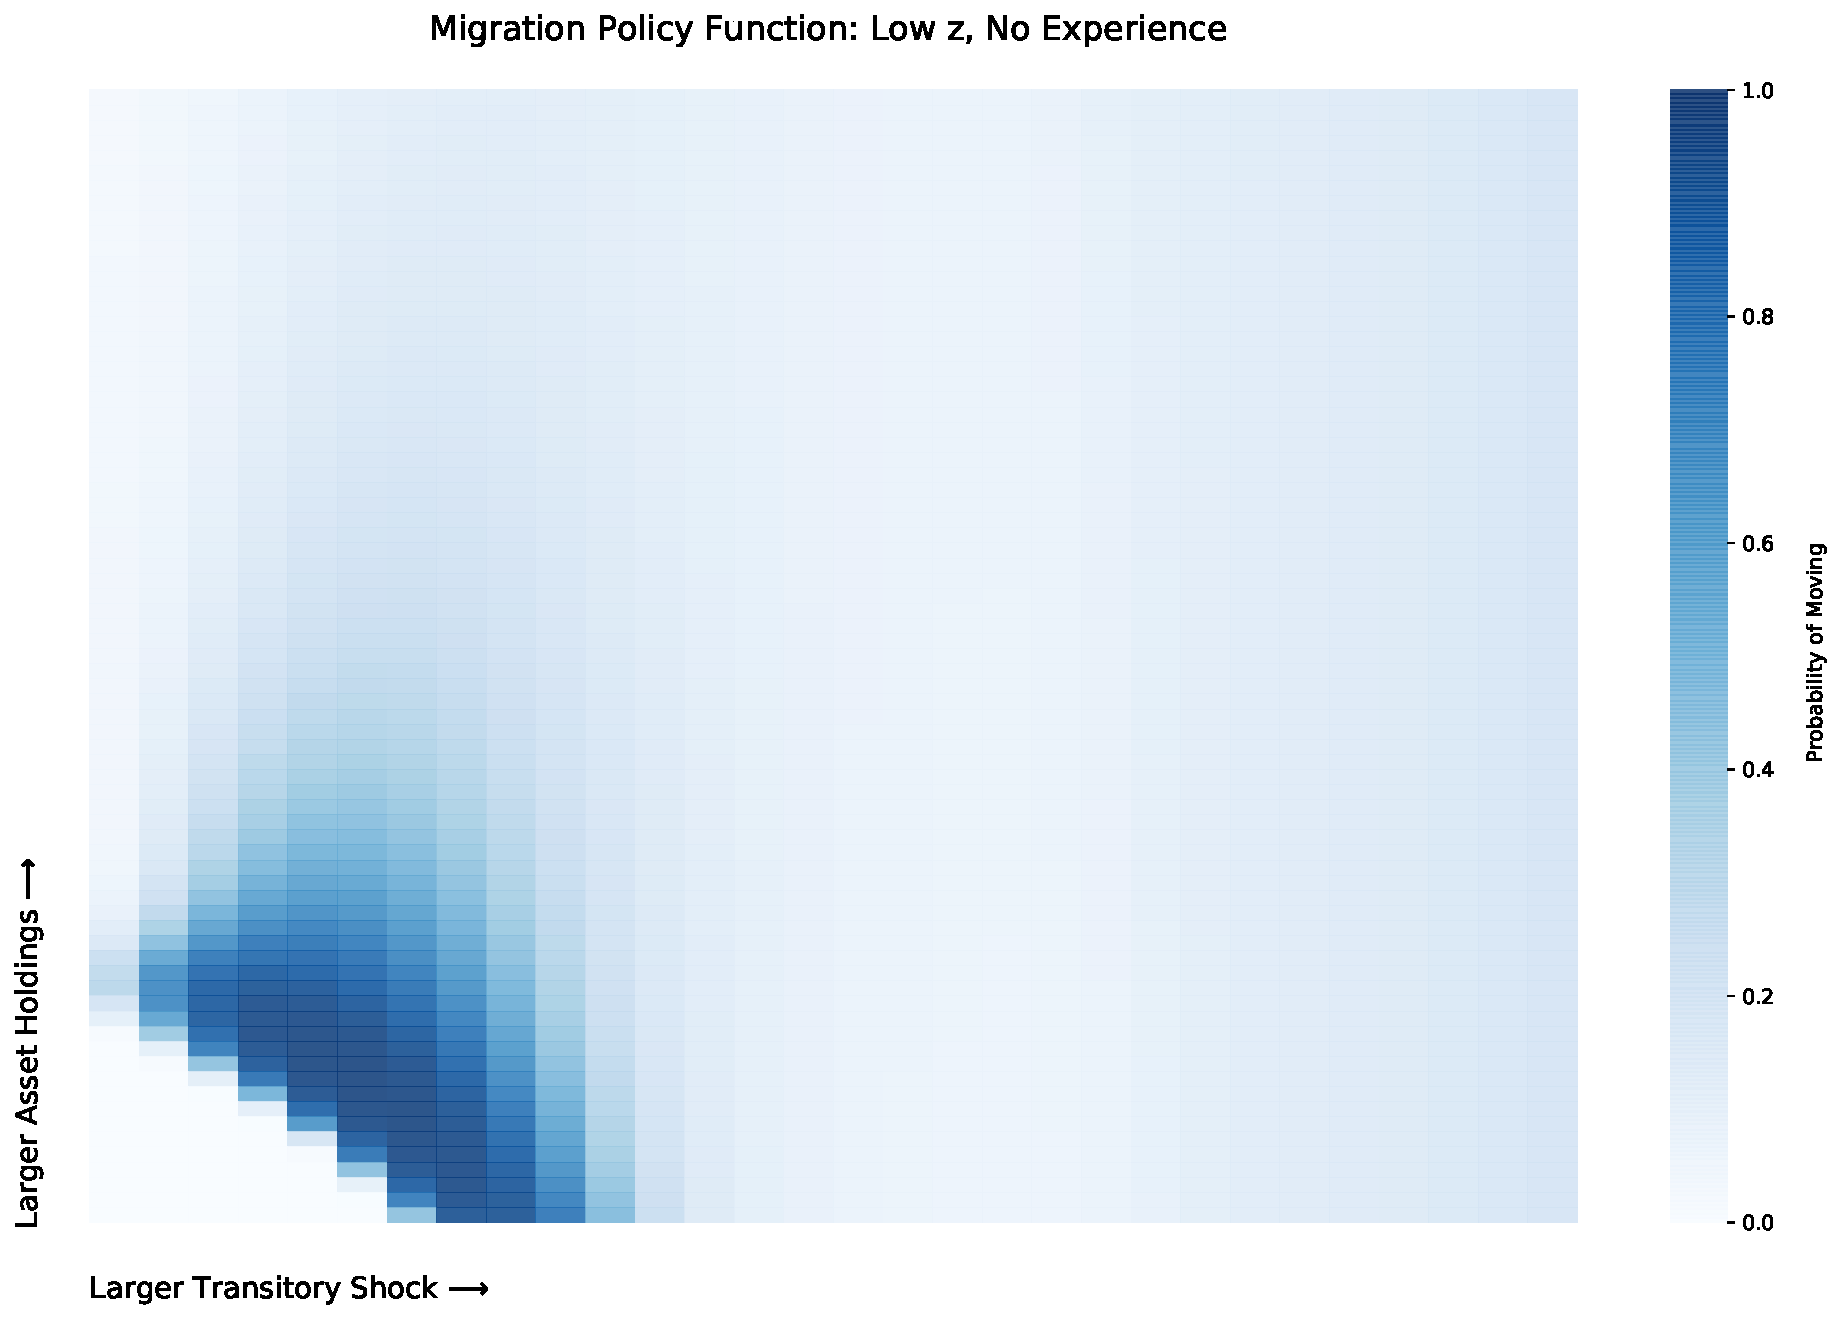
\includegraphics[scale = 0.37]{../figures/migration_policy_low_z.pdf}}
\end{figure}
\end{frame}
%
\begin{frame}[t]{Migration Policy: Moderate $z$, Lean Season, No Experience}
\begin{figure}[t]
\centerline{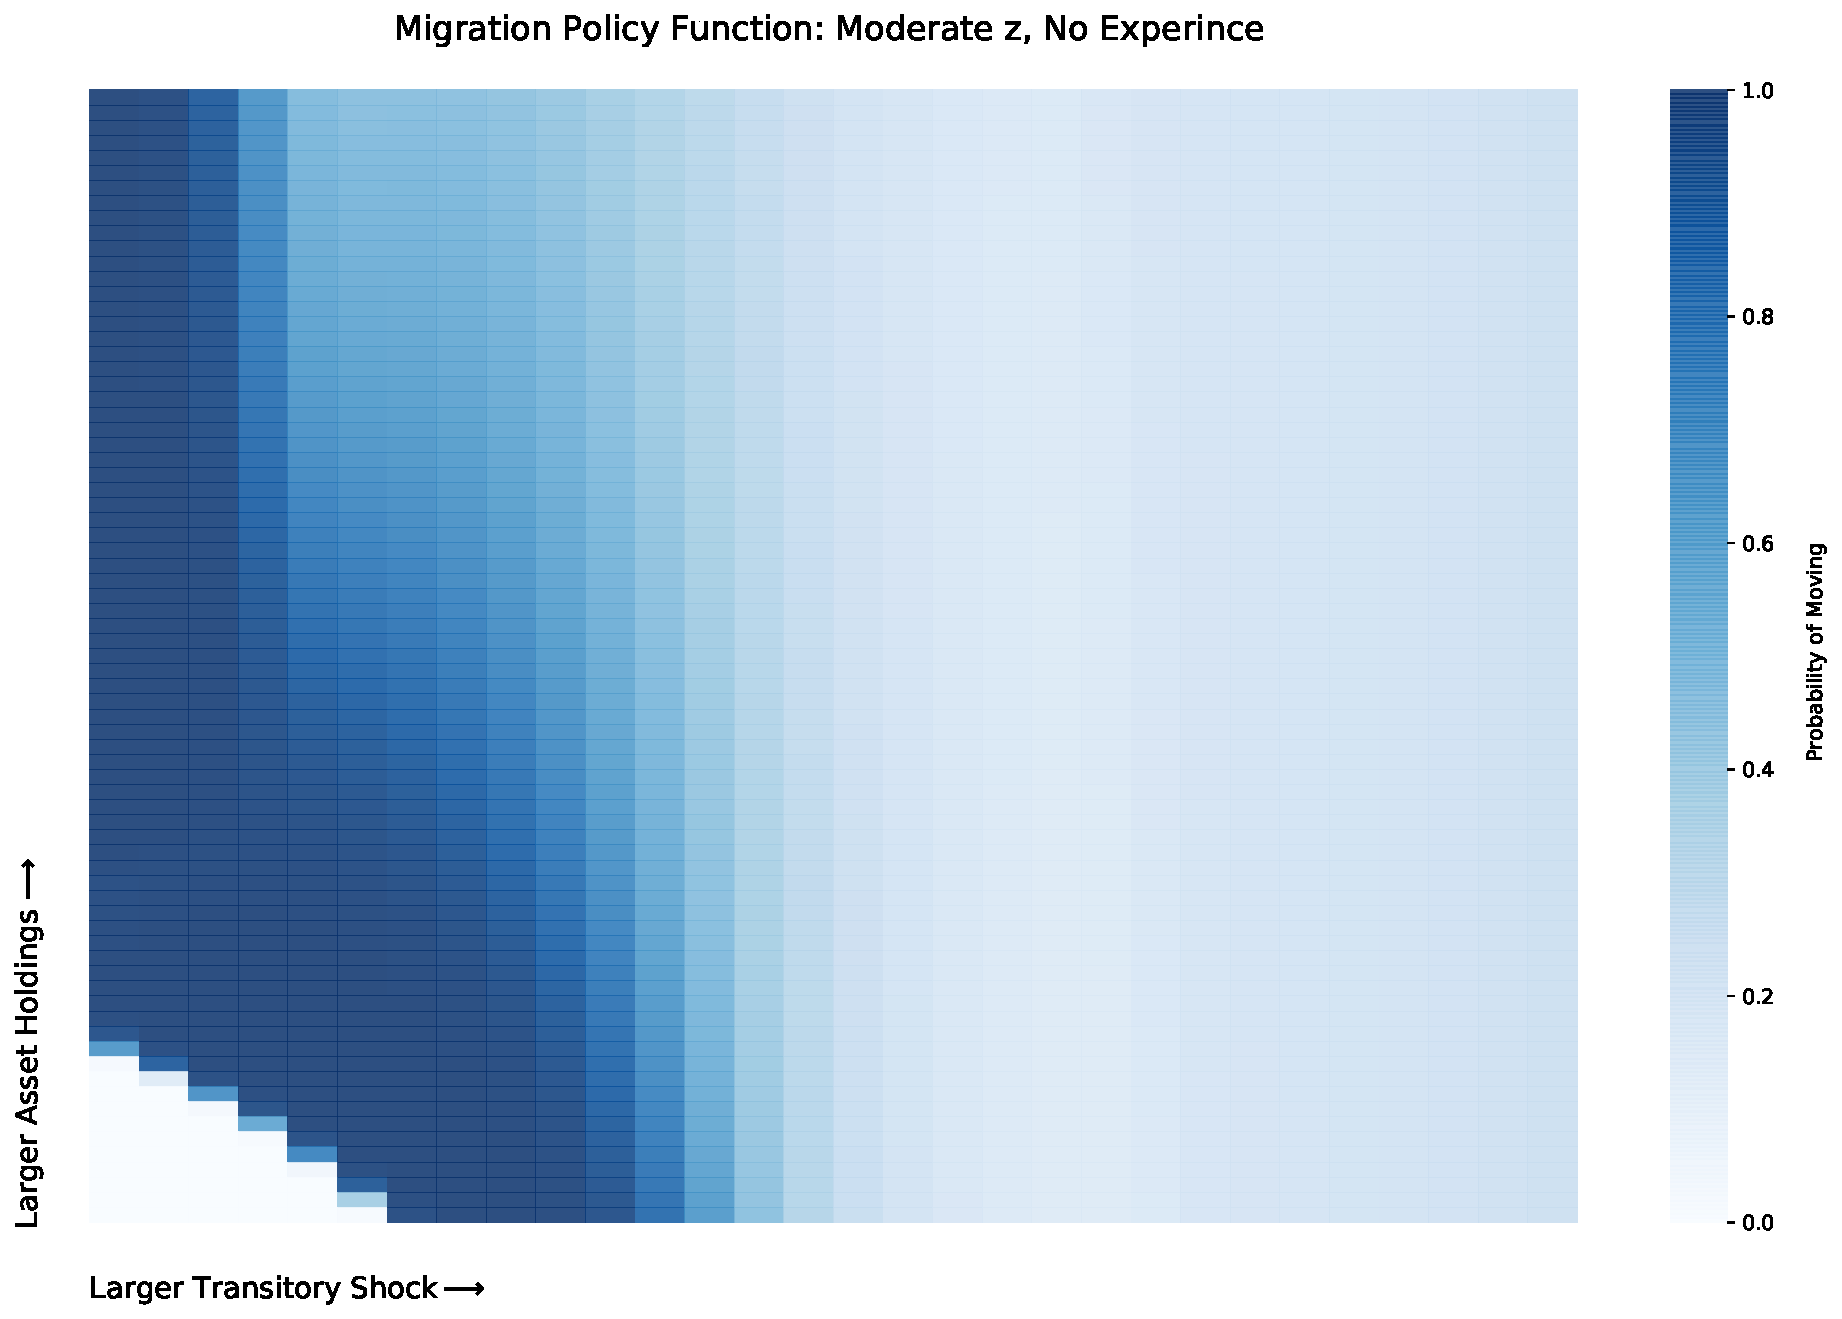
\includegraphics[scale = 0.37]{../figures/migration_policy_mod_z.pdf}}
\end{figure}
\end{frame}
%
\begin{frame}[t]{Migration Policy: Low $z$, Lean Season, Experience}
\begin{figure}[t]
\centerline{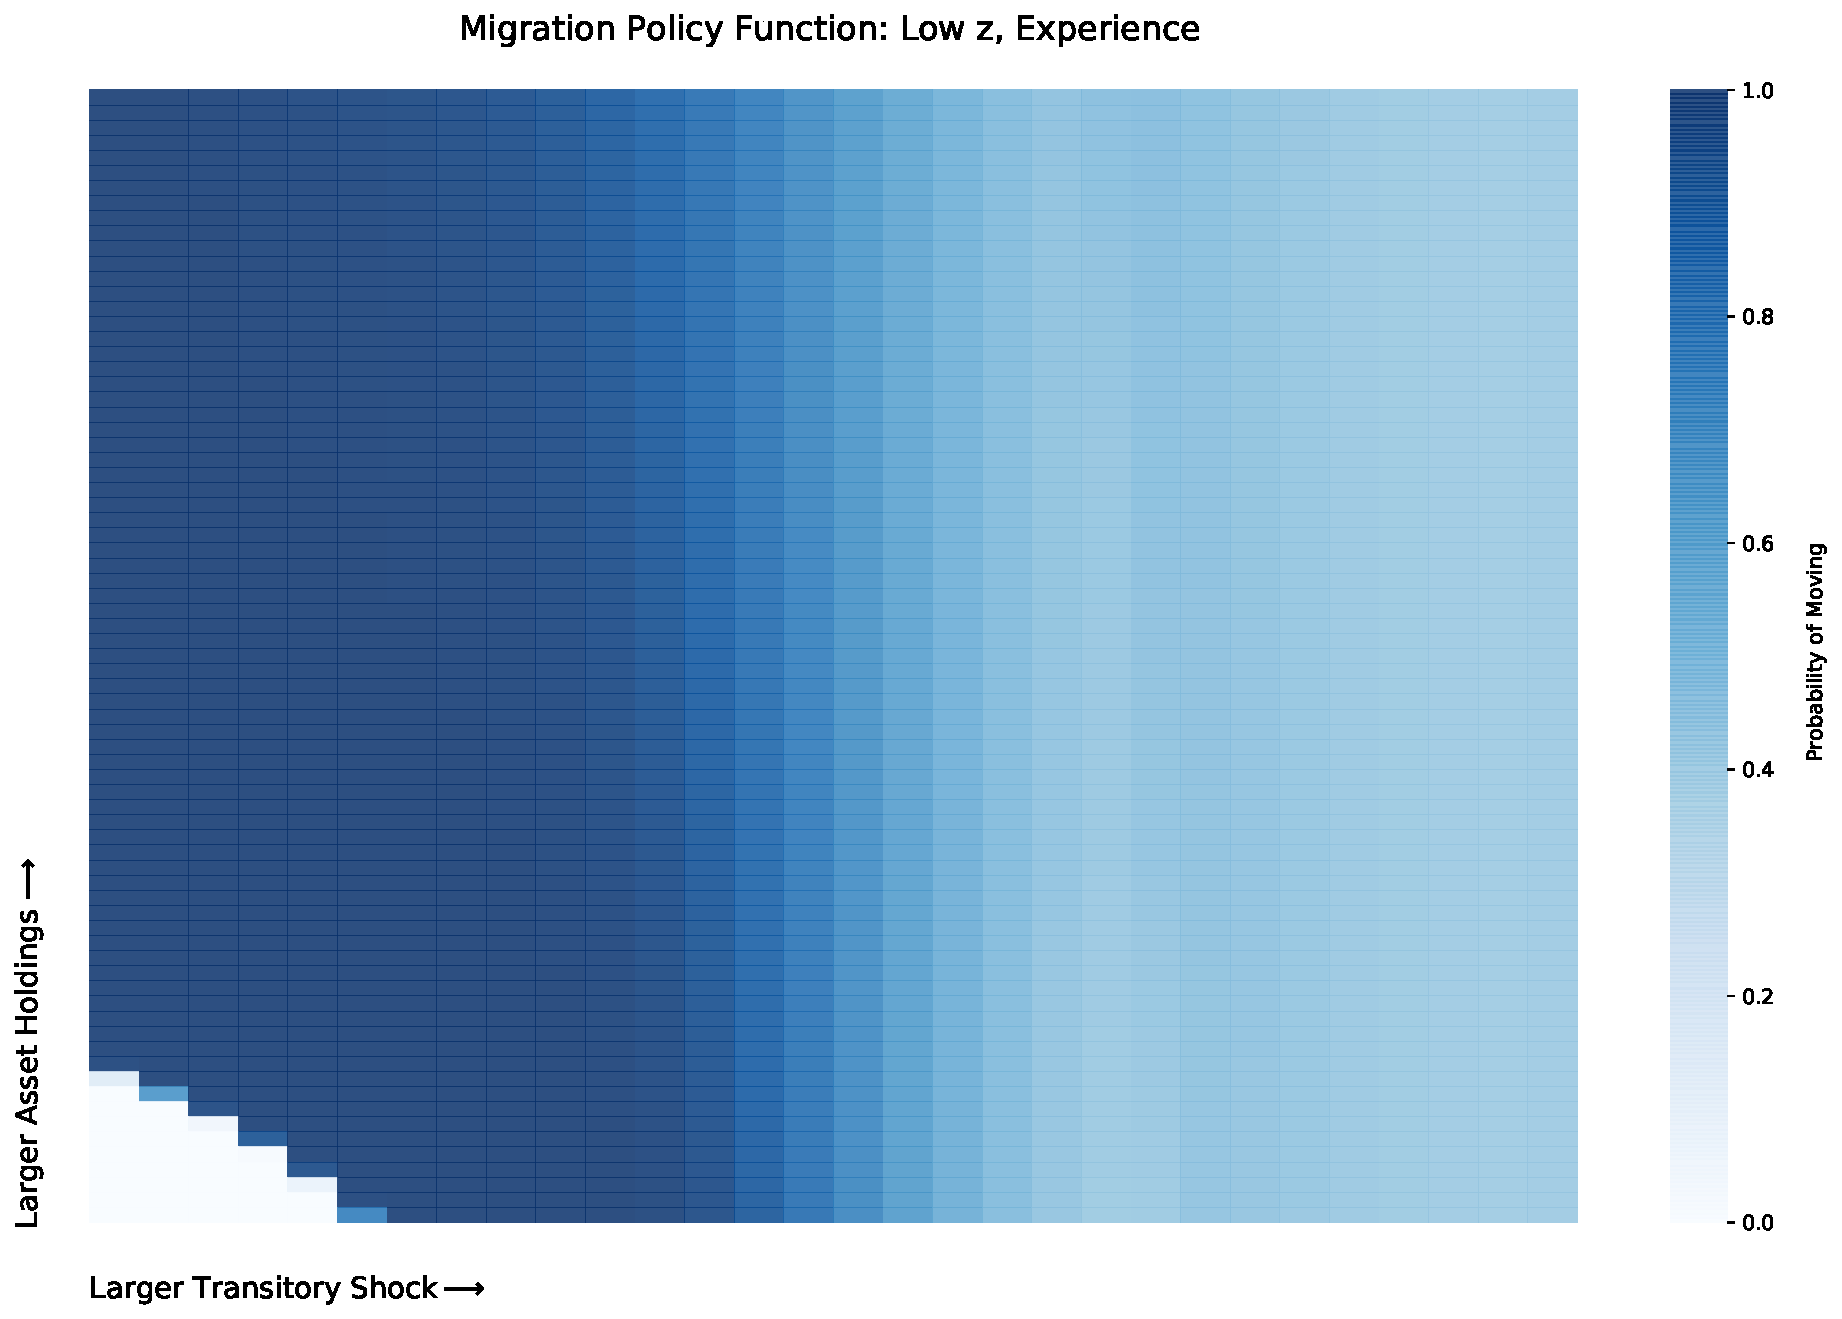
\includegraphics[scale = 0.37]{../figures/migration_policy_exp_z.pdf}}
\end{figure}
\end{frame}

\begin{frame}[t]{Control vs. Experiment: Low $z$, Lean Season, No Experience}
\begin{figure}[t]
\centerline{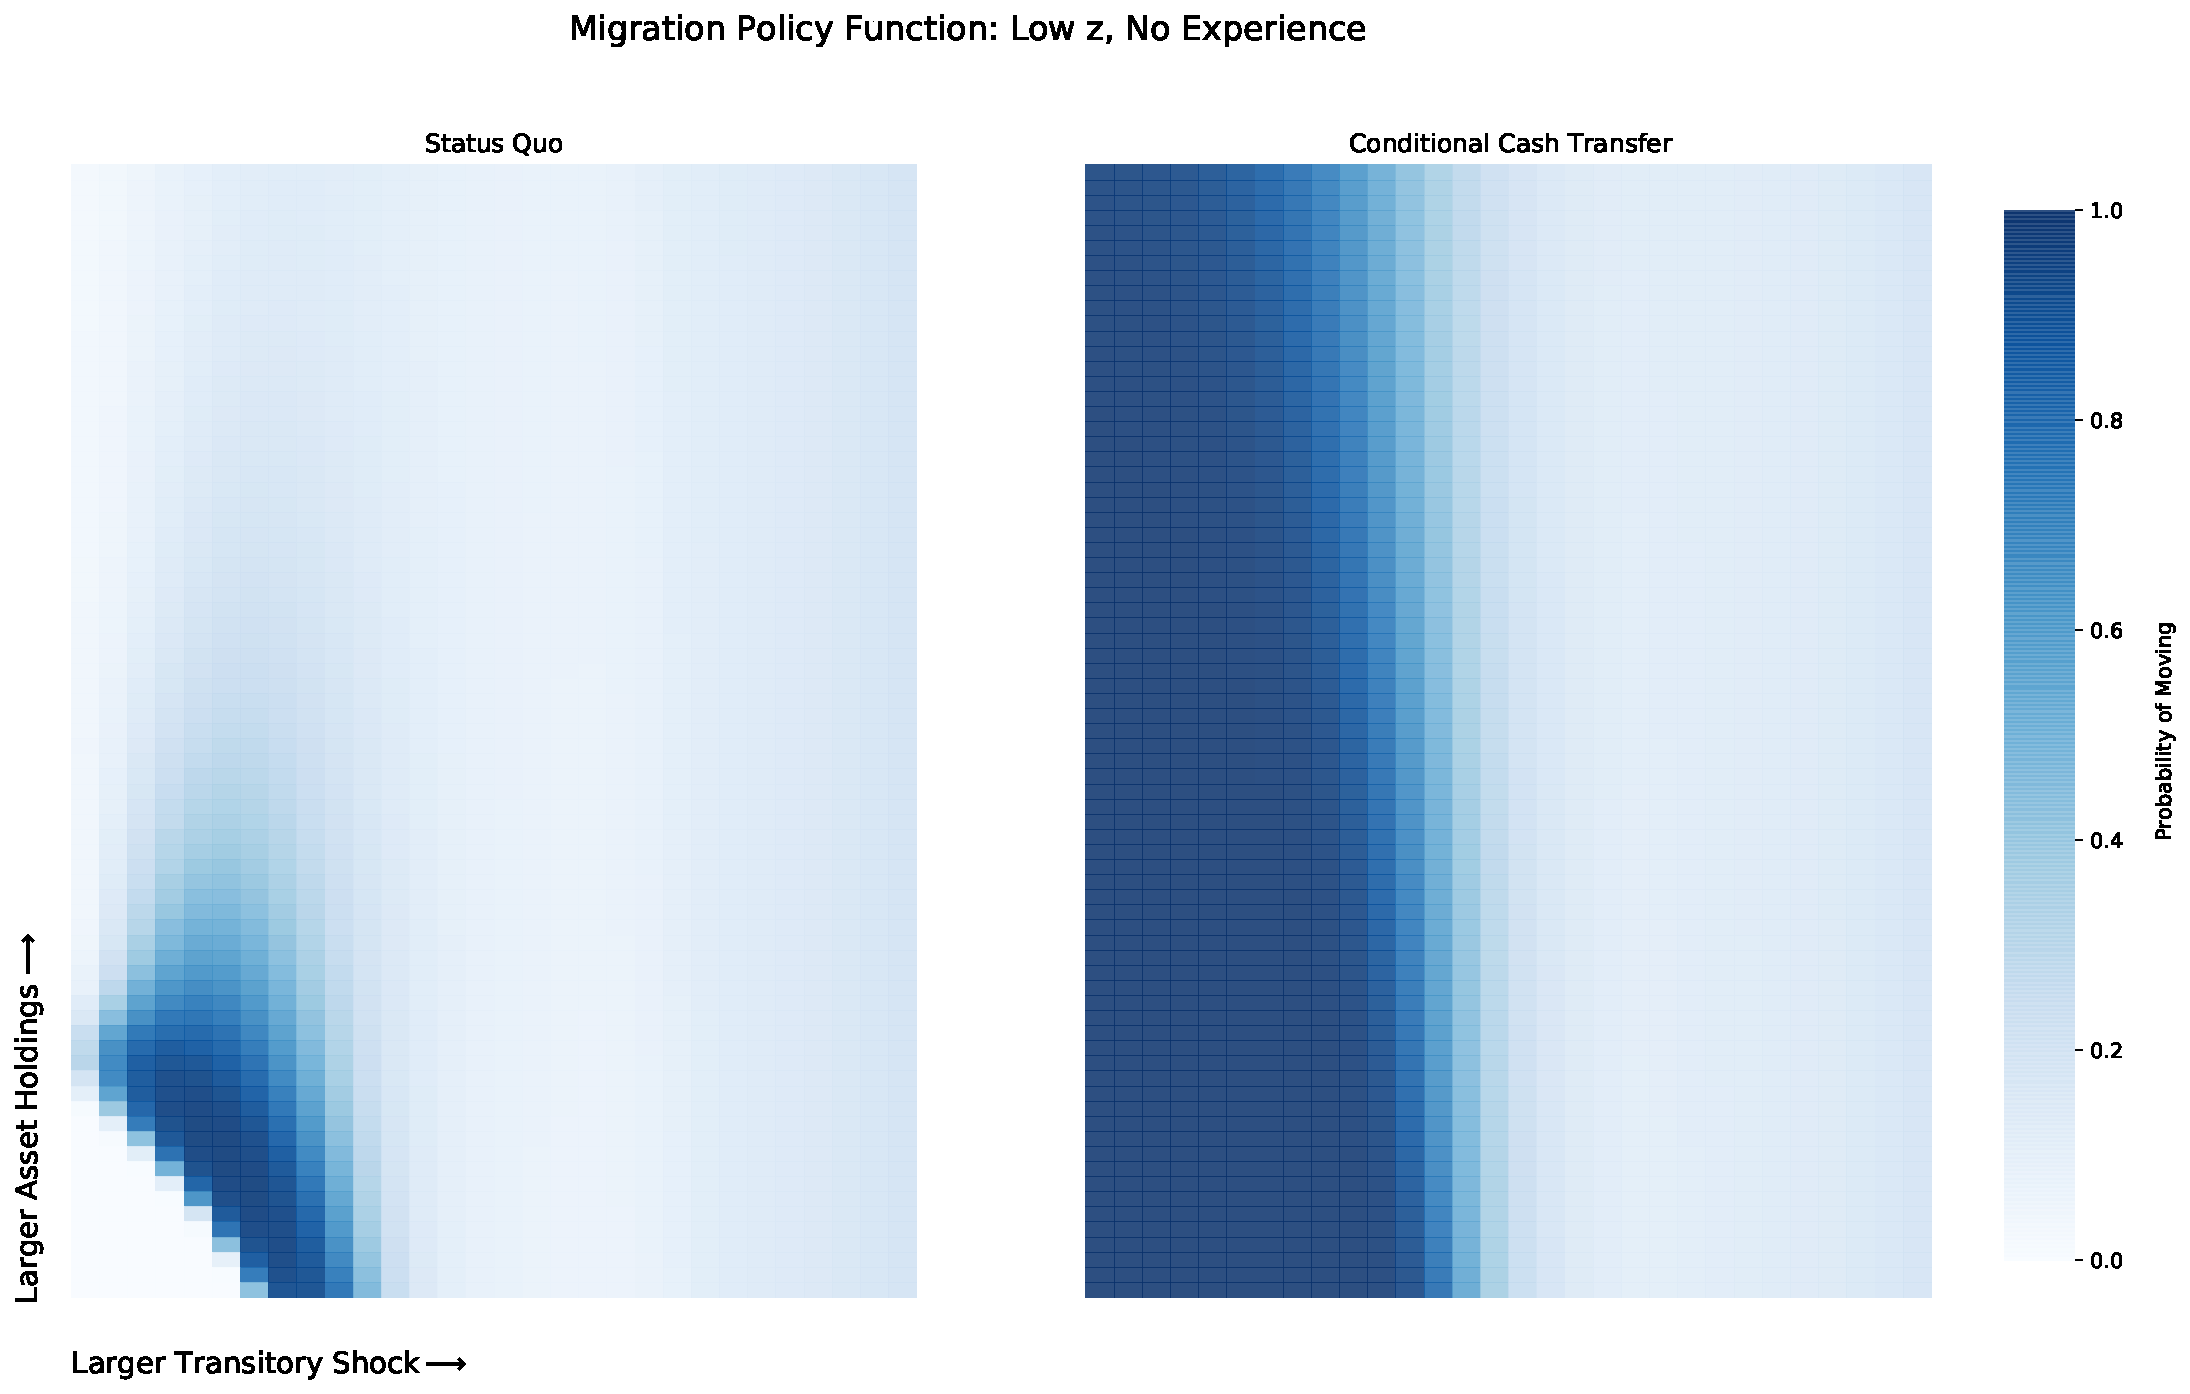
\includegraphics[scale = 0.35]{../figures/migration_policy_low_z_both.pdf}}
\end{figure}
\end{frame}

%%%%%%%%%%%%%%%%%%%%%%%%%%%%%%%%%%%%%%%%%%%%%%%%%%%%%%%%%%%%%%%%%%%%%%%%%%%%%%%%%%%%%%%%%%%%%%%%%
%%%%%%%%%%%%%%%%%%%%%%%%%%%%%%%%%%%%%%%%%%%%%%%%%%%%%%%%%%%%%%%%%%%%%%%%%%%%%%%%%%%%%%%%%%%%%%%%%

\begin{frame}[t]{Pause and Recap}
\textbf{1.} What happened in the experiment?
\begin{itemize}
\smallskip
\item In bad states of the world, urban migration is relatively more beneficial $\Rightarrow$ migration is insurance. 
\smallskip
\item And negative selection (LATE $>$ OLS) in the data reveals this. 
\end{itemize}
\bigskip
\uncover<2>{\textbf{2.} What are the welfare gains from conditional migration subsidies?} \\
\uncover<.>{
\begin{itemize}
\smallskip
\item Gains because they target those who need transfers the most, even if tax financed.  
\smallskip
\end{itemize}
\bigskip
\textbf{3.} What is the socially optimal outcome? \\
\begin{itemize}
\item Directly provide insurance with \textbf{less} movement of households across locations. 
\smallskip
\end{itemize}}
\end{frame}
%%%%%%%%%%%%%%%%%%%%%%%%%%%%%%%%%%%%%%%%%%%%%%%%%%%%%%%%%%%%%%%%%%%%%%%%%%%%%%%%%%%%%%%%%%%%%%%%%
%%%%%%%%%%%%%%%%%%%%%%%%%%%%%%%%%%%%%%%%%%%%%%%%%%%%%%%%%%%%%%%%%%%%%%%%%%%%%%%%%%%%%%%%%%%%%%%%%

\begin{frame}[t]{Welfare Gains: One-time Partial Equilibrium}
\vspace{-0.25cm}
\begin{table}[!t]
\small
\setlength {\tabcolsep}{1.55mm}
\renewcommand{\arraystretch}{1.30}
\begin{center}
\begin{tabular}{c c c c c c c c c c c}
\multicolumn{6}{l}{\textbf{Welfare Effects of Conditional Migration Subsidies}} \\
\hline
\hline
& & \multicolumn{2}{c}{Migration Subsidy} && \multicolumn{2}{c}{Migration Subsidy} && \multicolumn{2}{c}{Unconditional Transfer} \\
& & \multicolumn{2}{c}{Migration Endogenous} && \multicolumn{2}{c}{Migration Policy Fixed} && \multicolumn{2}{c}{Migration Endogenous}\\
\cmidrule(lr){3-4} \cmidrule(lr){5-7}     \cmidrule(lr){8-10}
& & \small Welfare  &\small Migr. Rate  && \small  Welfare  &\small Migr. Rate && \small  Welfare  &\small Migr. Rate \\
\multirow{5}{*}{\rotatebox{90}{\small Income Quintile}} & 1 & 1.16  & 85 && 0.76 & 48 && 1.05 & 45 \\
                                                       				 & 2 & 0.45  & 63 && 0.31 & 38 && 0.56 & 37 \\
                                                        				& 3 & 0.28  & 51 && 0.20 & 33 && 0.40 & 33 \\
                                                       				 & 4 & 0.20  & 46 && 0.15 & 31 && 0.32 & 31 \\
                                                      				  & 5 & 0.12  & 41 && 0.10 & 31 && 0.20 & 31 \\
\hline
\multicolumn{2}{l}{\small \underline{Average}}      &  & &&  & &&   &  \\
\multicolumn{2}{l}{\small Rural \& Access to Subsidy}      &0.44  & 57 && 0.30 & 36 &&  0.51 &  35 \\
\multicolumn{2}{l}{\small All Rural}      &0.22  & 44 && 0.15 & 31 &&  0.25 &  33 \\
\hline
\end{tabular}
\parbox[c]{5.45in}{%
{\footnotesize  \vspace{0.1cm} \textbf{Note:} The table reports the lifetime consumption-equivalent welfare gains to rural assets with low assets from one-time conditional migration subsidies and from a one-time unconditional transfer. The rows are for different income quintiles of the rural households eligible for the subsidy, who are those in the bottom half of the rural asset distribution, with 1 being the poorest quintile and 5 being the richest.}
}
\end{center}
\end{table}
\end{frame}

%%%%%%%%%%%%%%%%%%%%%%%%%%%%%%%%%%%%%%%%%%%%%%%%%%%%%%%%%%%%%%%%%%%%%%%%%%%%%%%%%%%%%%%%%%%%%%%%
%%%%%%%%%%%%%%%%%%%%%%%%%%%%%%%%%%%%%%%%%%%%%%%%%%%%%%%%%%%%%%%%%%%%%%%%%%%%%%%%%%%%%%%%%%%%%%%%

\begin{frame}[t]{Welfare Gains: Permanent, Tax Financed, General Equilibrium}
\vspace{-0.25cm}
\begin{table}[!t]
\small
\setlength {\tabcolsep}{2.055mm}
\renewcommand{\arraystretch}{1.30}
\begin{center}
\begin{tabular}{l c c c}
\multicolumn{4}{l}{\textbf{Welfare Effects of Permanent Migration Subsidies}} \\
\hline
\hline
						& Migration Fixed & Migration Fixed & Migration Endogenous \\
						& No Taxation & Tax Financed & Tax Financed (G.E.) \\
						\cmidrule(lr){2-2} \cmidrule(lr){3-3}     \cmidrule(lr){4-4}
%\underline{Average Welfare Gain}      & 		&  			&  \\
Rural \& Access to Subsidy      & \textbf{3.00}  			& \textbf{2.00} 			& \textbf{1.50}  \\
All Rural      &1.48  			& 1.07 			& 1.55  \\
All Urban     & 0.11 			& -0.31 			& -1.14  \\
All Households      & 0.93  			& 0.59 			& 0.63  \\
\hline
Percent in Rural Area				   & 60 			& 60				&  66 \\
Percent of Rural Seasonally Migrating		   & 31 			& 31				&  69 \\
Percent of Rural with Access to Subsidy		   & 50 			& 50				&  72 \\
Tax Rate (\% of labor income)		  		 & 0 			& 0.4				&  1.2 \\
%\multicolumn{2}{l}{\small Fraction w. Experience} &  &23 &&  &42&&   &  41\\
\hline
\end{tabular}
\parbox[t]{5.25in}{%
{\footnotesize  \vspace{0.1cm} \textbf{Note:} The first column reports the effects of permanently offering conditional migration subsidies to rural households with sufficiently low assets, as in the migration experiments, but holding migration policies fixed and without any taxation to pay for the transfers. The second column is the same but financing the migration subsidies through labor taxation. The third column considers the full effects of the migration transfers, where migration responds endogenously and the migration subsides are financed through labor taxation.}
}
\end{center}
\end{table}
\end{frame}

\begin{frame}[t]{Pause and Recap}
\uncover<.>{\textbf{1.} What happened in the experiment?
\begin{itemize}
\smallskip
\item In bad states of the world, urban migration is relatively more beneficial $\Rightarrow$ migration is insurance.
\smallskip
\item And negative selection (LATE $>$ OLS) in the data reveals this.
\end{itemize}}
\bigskip
\uncover<1>{\textbf{2.} What are the welfare gains from conditional migration subsidies? \\
\begin{itemize}
\smallskip
\item Gains because they target those who need transfers the most, even if tax financed.
\smallskip
\end{itemize}}
\bigskip
\uncover<2>{\textbf{3.} What is the socially optimal outcome?} \\
\uncover<.>{
\begin{itemize}
\item Directly provide insurance with \textbf{less} movement of households across locations.
\smallskip
\end{itemize}}
\end{frame}

%%%%%%%%%%%%%%%%%%%%%%%%%%%%%%%%%%%%%%%%%%%%%%%%%%%%%%%%%%%%%%%%%%%%%%%%%%%%%%%%%%%%%%%%%%%%%%%%
%%%%%%%%%%%%%%%%%%%%%%%%%%%%%%%%%%%%%%%%%%%%%%%%%%%%%%%%%%%%%%%%%%%%%%%%%%%%%%%%%%%%%%%%%%%%%%%%

\begin{frame}[t]{The Planners Problem}
Choose migration rates $\mu_{j'j}$ and consumption for all source $j$ and destination $j'$ pairs, states, and dates:\\
\begin{align}
\small
& \max \ \sum_{t=0}^{\infty}\sum_{j} \int\limits_{z} \int\limits_{s} \int\limits_{x} \beta^{t} \bigg \{ u(c_{j',j}(z, s, x, t), x) + E[ \nu \ | \big\{ \mu_{j',j}(z,s,x,t)\big\}_{j'}] \bigg \} \lambda_{j}(z, s, x, t) \ dz \ ds \ dx \nonumber \\[.75em]
& \mbox{subject to} \nonumber\\[.75em]
& \ \ \ \ \mbox{feasibility} \ \ \ [\ \mathbf{\chi(t)} \ ], \nonumber \\[.75em]
& \ \ \ \ \mbox{law of motion on the probability mass of hh,} \ \lambda_j(z, s, x, t) \ \ \ [\ \mathbf{\chi_{3j}(z, s, x, t)} \ ], \nonumber \\[.75em]
& \ \ \ \ \mbox{migration probabilities}, \ \ \sum_{j'} \mu_{j',j}(z, s, x,t) = 1,  \ \ \ \ [\ \mathbf{\chi_{2j}(z, s, x, t)} \ ], \nonumber \\[.75em]
& \ \ \ \ \mbox{and an inital condition}, \ \ \ \ \lambda_j(z, s, x,0). \nonumber
\end{align}
\end{frame}

%%%%%%%%%%%%%%%%%%%%%%%%%%%%%%%%%%%%%%%%%%%%%%%%%%%%%%%%%%%%%%%%%%%%%%%%%%%%%%%%%%%%%%%%%%%%%%%%
%%%%%%%%%%%%%%%%%%%%%%%%%%%%%%%%%%%%%%%%%%%%%%%%%%%%%%%%%%%%%%%%%%%%%%%%%%%%%%%%%%%%%%%%%%%%%%%%

\begin{frame}[t]{The Efficient Allocation}
\textbf{Proposition 1: Efficient Consumption and Migration} Consumption allocations equate the marginal utility of consumption in all locations, productivity and experience states for each date $t$:
\vspace{0.15cm}
{\small
\begin{align}
u'(t) = u'(c_{j',j}(z, s, x, t)) = u'(c_{\tilde{j'},\tilde{j}}(z, s', x', t)) \ \ \ \forall \ j, \ z , \ s, \ x  \nonumber \\[.75em] \nonumber
\end{align}
}
Migration probabilities  $\mu_{j'j}(z,s,x,t)$ satisfy:
\vspace{0.25cm}
{\small
\begin{align}
\exp \left(\frac{- u'(t) \ m_{j',j} + \beta \ \mathbb{E}_{s,x}\left[\chi_{3j'}(z,s,x, t+1)\right]}{\sigma} \right)  \Bigg / \sum_{j'} \exp \left( \frac{- u'(t)\ m_{j',j} + \beta \  \mathbb{E}_{s,x}\left[\chi_{3j'}(z,s,x, t+1) \right]}{\sigma} \right), \nonumber \\[.75em] \nonumber
\end{align}
}
with the multipliers $\chi_{3j'}$ satisfying the following recursive relationship
\vspace{0.15cm}
{\small
\begin{align}
& \ \ \chi_{3j'}(z, s, x, t+1) =  u_{j'}(x, t+1) +  u'(t+1) \kappa_{j'}(z, s,x,t+1) + \beta \mathbb{E}\left[\chi_{3}(z,s,x, t+2) \right], \nonumber
\end{align}}
where
\vspace{0.15cm}
{\small
\begin{align}
& \ \ \kappa_{j'}(z, s',x',t+1) = \mbox{\texttt{mpl}}_{j'}(z,s',t+1) - c(z, s',x',t+1) - \sum_{j''}  m_{j'',j'} \ \mu_{j'',j'}(z, s', x', t+1). \nonumber
\end{align}}
\end{frame}

%%%%%%%%%%%%%%%%%%%%%%%%%%%%%%%%%%%%%%%%%%%%%%%%%%%%%%%%%%%%%%%%%%%%%%%%%%%%%%%%%%%%%%%%%%%%%%%%
%%%%%%%%%%%%%%%%%%%%%%%%%%%%%%%%%%%%%%%%%%%%%%%%%%%%%%%%%%%%%%%%%%%%%%%%%%%%%%%%%%%%%%%%%%%%%%%%

\begin{frame}[t]{The Efficient Allocation in Words}
What the planner does:\\
\bigskip
\textbf{1.} Equate the marginal utility of consumption across locations and states|full risk sharing result.\\
\bigskip
\textbf{2.} Dynamically move households based on current costs and future net social benefits:
\begin{itemize}
\smallskip
\item current costs: the moving costs evaluated at the marginal utility of consumption.
\smallskip
\item Future net social benefits:\\
\smallskip
how much utility a household gets and their marginal product of labor, net of...\\
\smallskip
the consumption cost to provide that utility and cost of moving elsewhere in the future,\\
\smallskip
plus the next periods discounted, expected future net social benefits.
\end{itemize}
\end{frame}

%%%%%%%%%%%%%%%%%%%%%%%%%%%%%%%%%%%%%%%%%%%%%%%%%%%%%%%%%%%%%%%%%%%%%%%%%%%%%%%%%%%%%%%%%%%%%%%%
%%%%%%%%%%%%%%%%%%%%%%%%%%%%%%%%%%%%%%%%%%%%%%%%%%%%%%%%%%%%%%%%%%%%%%%%%%%%%%%%%%%%%%%%%%%%%%%%


\begin{frame}[t]{The Efficient Allocation}
\begin{table}[!t]
\small
\setlength {\tabcolsep}{2.055mm}
\renewcommand{\arraystretch}{1.40}
\begin{center}
\begin{tabular}{l c c c}
\multicolumn{4}{l}{\textbf{Competitive Equilibrium vs Social Planner's Allocation}} \\
\hline
\hline
						& Competitive & Full Insurance & Full Insurance  \\
						& Equilibrium & Migration Fixed & Migration Endogenous \\
						\cmidrule(lr){2-2} \cmidrule(lr){3-3}     \cmidrule(lr){4-4}
Average Welfare Gain  (\%, Relative to C.E.)      & ---   			& 46.5 			& 48.0  \\
Percent in Rural Area				   & 60 			& 60				&  53 \\
Percent of Rural Seasonally Migrating		   & 31 			& 31				&  27 \\
Rural-Urban Wage Gap				   & 1.88 			& 1.88				&  1.56 \\
\hline
\hline
\end{tabular}
\parbox[c]{5.2in}{%
{\footnotesize  \vspace{0.1cm} \textbf{Note:} The first column reproduces features of the competitive-equilibrium outcome. The second column reports the welfare gains from moving to an allocation with full consumption insurance but holding migration policies fixed, and features of this allocation. The third column reports the welfare gains from moving to the efficient allocation, with full consumption insurance and allowing for endogenous migration decisions, and features of this allocation.}
}
\end{center}
\end{table}
\end{frame}

%%%%%%%%%%%%%%%%%%%%%%%%%%%%%%%%%%%%%%%%%%%%%%%%%%%%%%%%%%%%%%%%%%%%%%%%%%%%%%%%%%%%%%%%%%%%%%%%%%
%%%%%%%%%%%%%%%%%%%%%%%%%%%%%%%%%%%%%%%%%%%%%%%%%%%%%%%%%%%%%%%%%%%%%%%%%%%%%%%%%%%%%%%%%%%%%%%%%%

\begin{frame}[t]{Status Quo vs. Efficient Migration: Low $z$, No Experience}
\begin{figure}[t]
\centerline{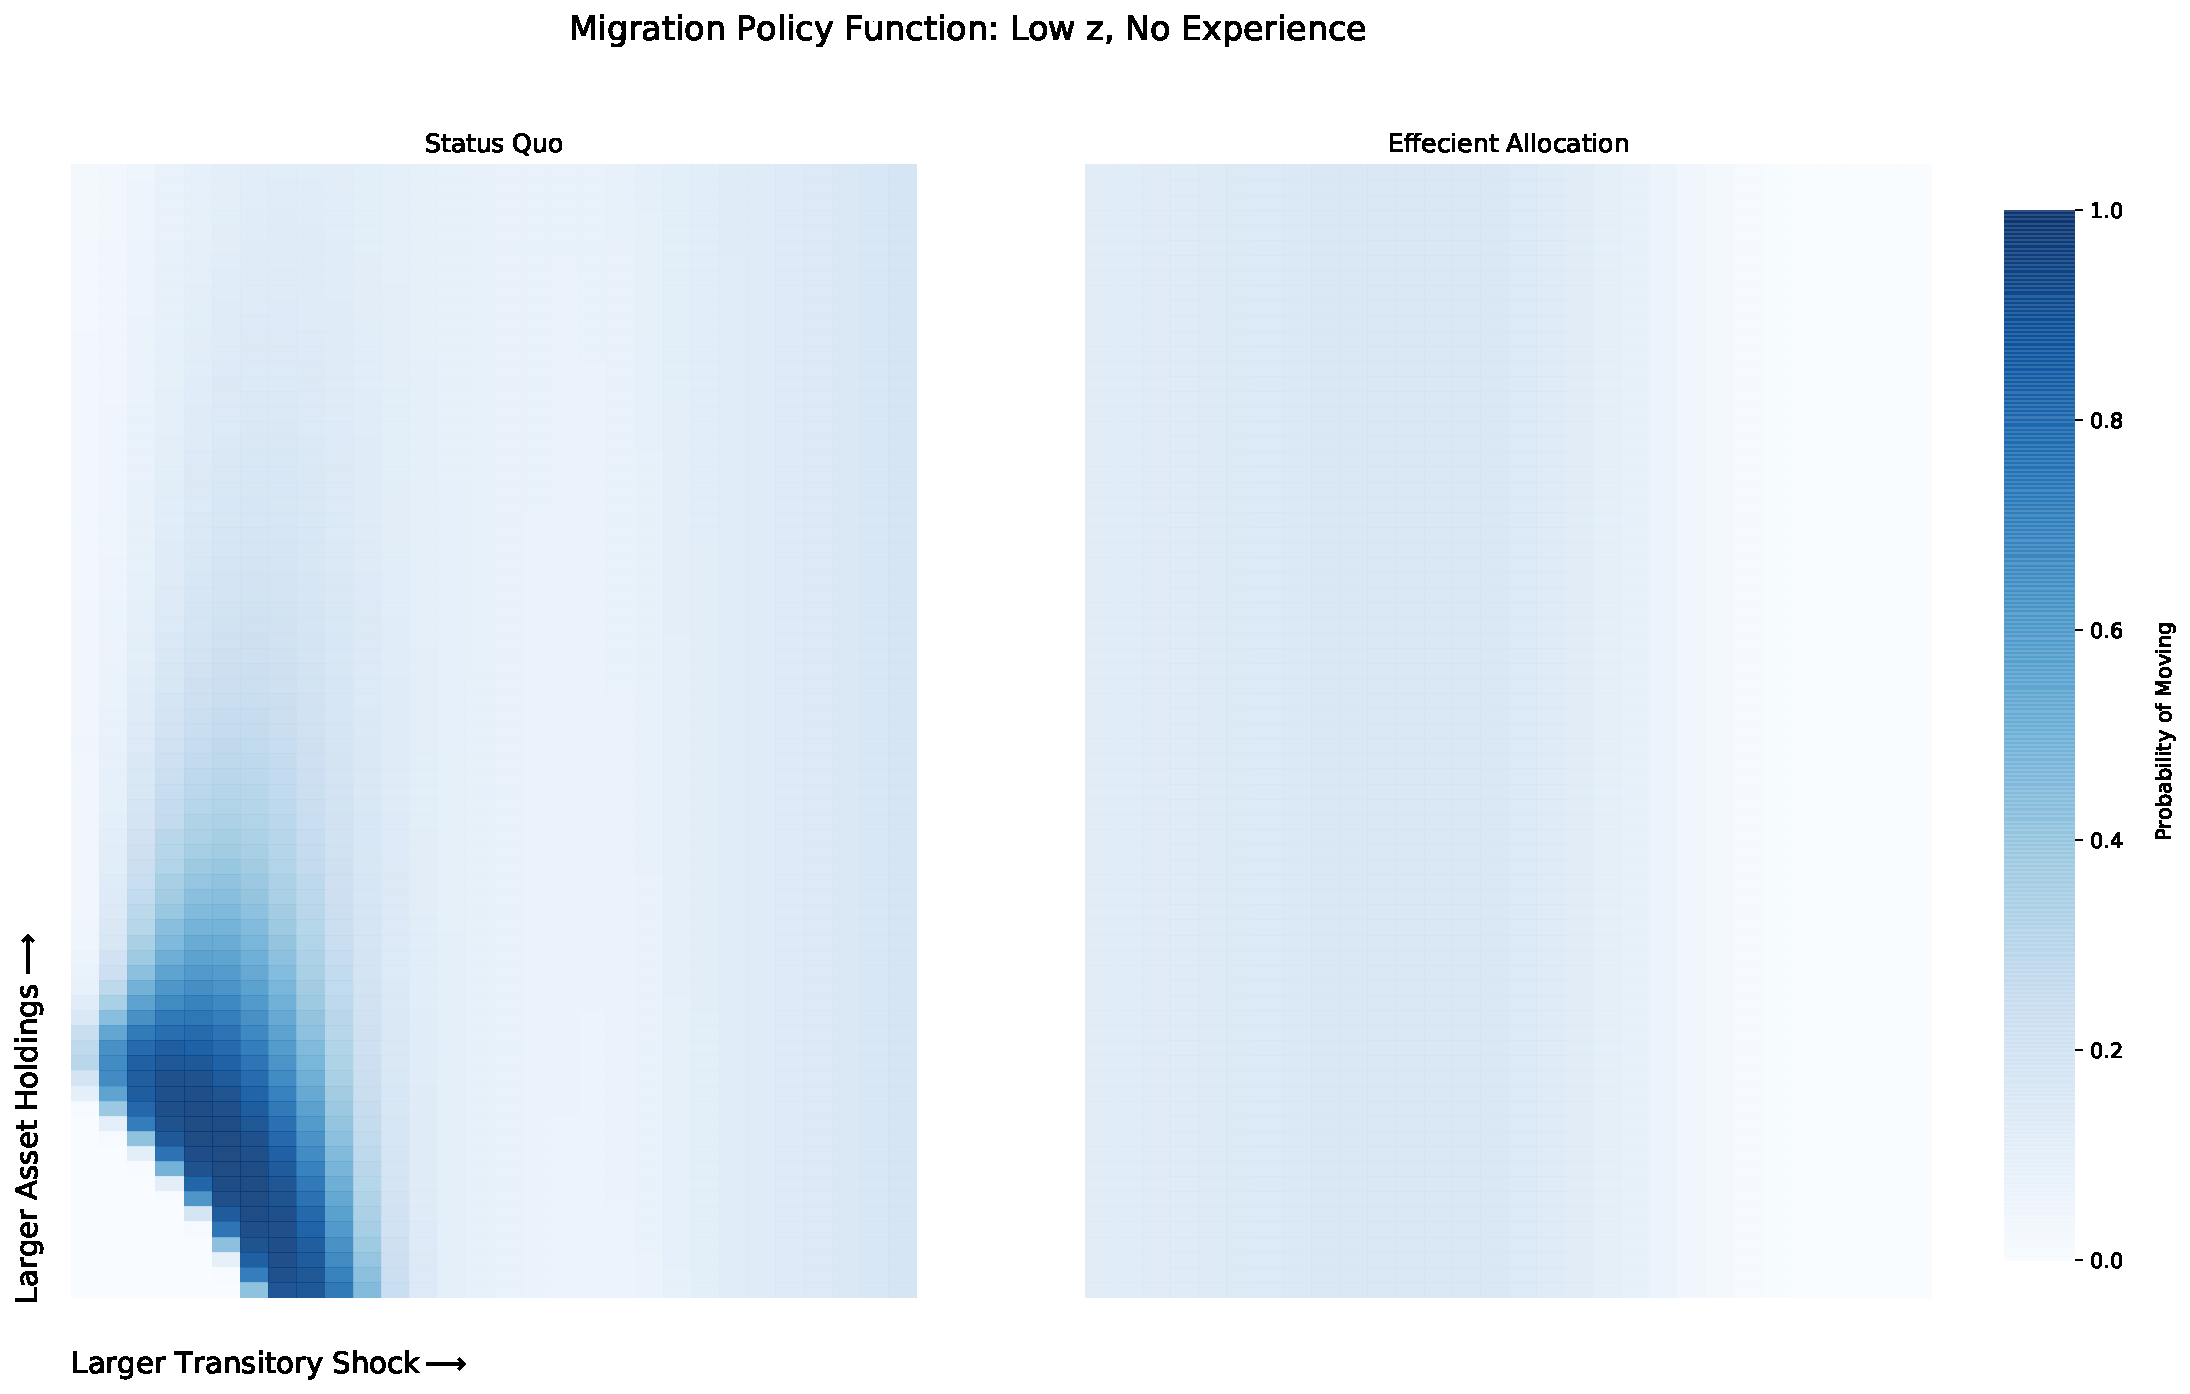
\includegraphics[scale = 0.37]{../figures/effecient_migration_policy_low_z_both.pdf}}
\end{figure}
\end{frame}

\begin{frame}[t]{Status Quo vs. Efficient Migration: Low $z$, Experience}
\begin{figure}[t]
\centerline{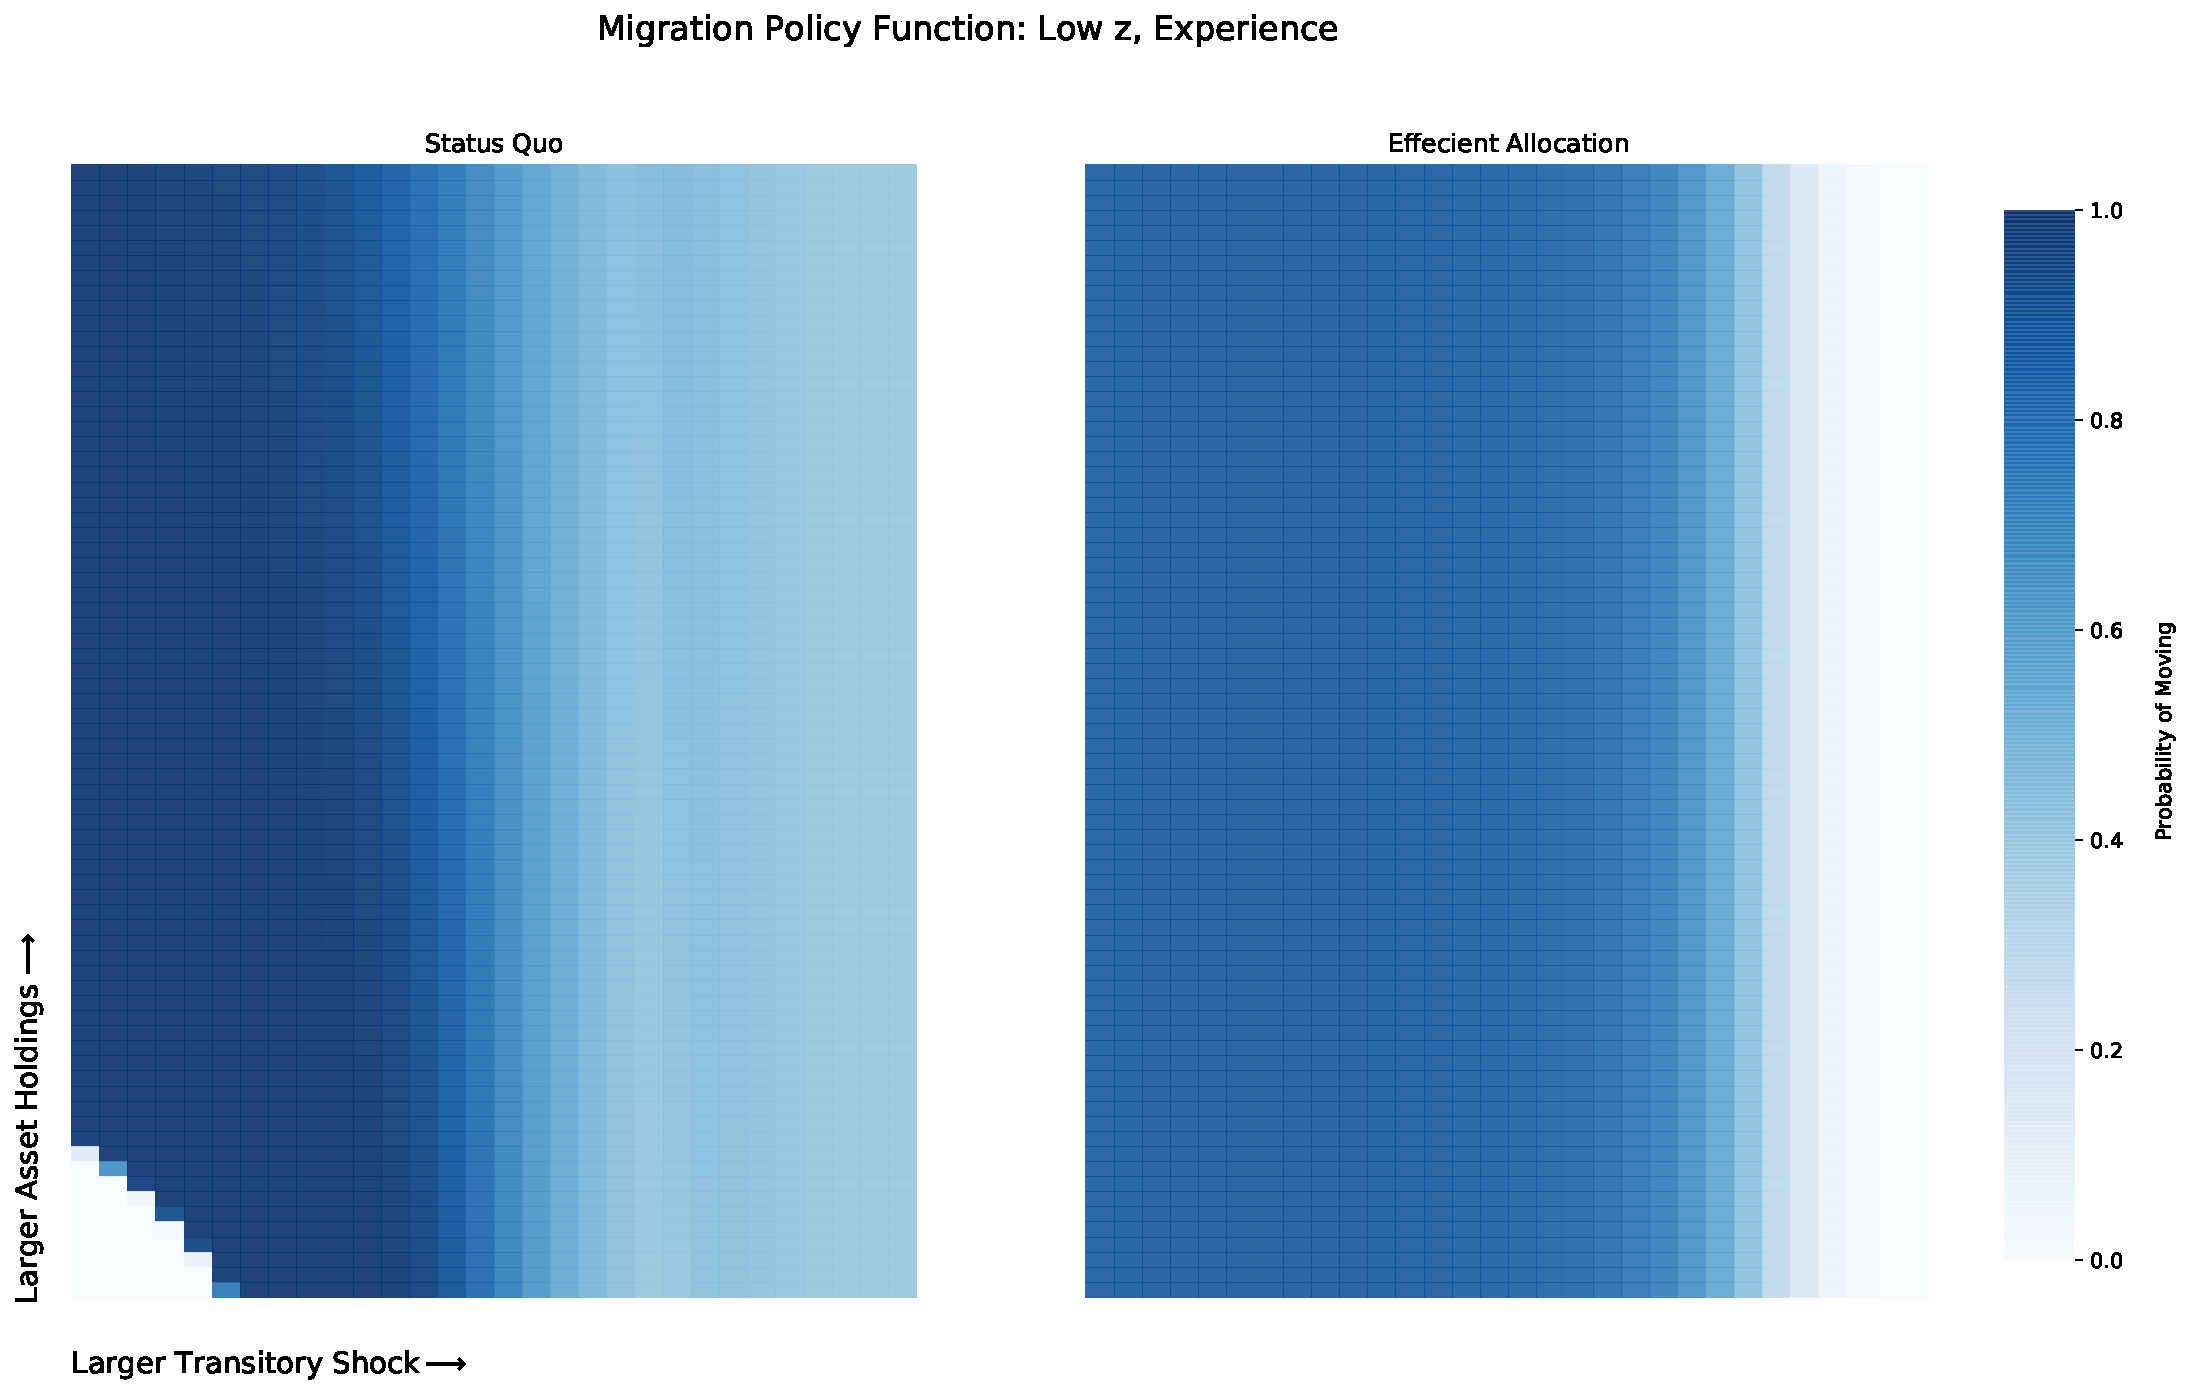
\includegraphics[scale = 0.37]{../figures/effecient_migration_policy_exp_z_both.pdf}}
\end{figure}
\end{frame}

%%%%%%%%%%%%%%%%%%%%%%%%%%%%%%%%%%%%%%%%%%%%%%%%%%%%%%%%%%%%%%%%%%%%%%%%%%%%%%%%%%%%%%%%%%%%%%%%
%%%%%%%%%%%%%%%%%%%%%%%%%%%%%%%%%%%%%%%%%%%%%%%%%%%%%%%%%%%%%%%%%%%%%%%%%%%%%%%%%%%%%%%%%%%%%%%%

\begin{frame}[t]{Conclusion\ldots}
\textbf{1.} What happened in the experiment?
\begin{itemize}
\smallskip
\item In bad states of the world, urban migration is relatively more beneficial $\Rightarrow$ migration is insurance.
\smallskip
\item And negative selection (LATE $>$ OLS) in the data reveals this.
\end{itemize}
\bigskip
\textbf{2.} What are the welfare gains from conditional migration subsidies? \\
\begin{itemize}
\smallskip
\item Gains because they target those who need transfers the most, even if tax financed.
\smallskip
\end{itemize}
\bigskip
\textbf{3.} What is the socially optimal outcome? \\
\begin{itemize}
\item Directly provide insurance with \textbf{less} movement of households across locations.
\smallskip
\end{itemize}
\end{frame}

%%%%%%%%%%%%%%%%%%%%%%%%%%%%%%%%%%%%%%%%%%%%%%%%%%%%%%%%%%%%%%%%%%%%%%%%%%%%%%%%%%%%%%%%%%%%%%%%
%%%%%%%%%%%%%%%%%%%%%%%%%%%%%%%%%%%%%%%%%%%%%%%%%%%%%%%%%%%%%%%%%%%%%%%%%%%%%%%%%%%%%%%%%%%%%%%%

\appendix

\newcounter{finalframe}
\setcounter{finalframe}{\value{framenumber}}

%%%%%%%%%%%%%%%%%%%%%%%%%%%%%%%%%%%%%%%%%%%%%%%%%%%%%%%%%%%%%%%%%%%%%%%%%%%%%%%%%%%%%%%%%%%%%%%%%
%%%%%%%%%%%%%%%%%%%%%%%%%%%%%%%%%%%%%%%%%%%%%%%%%%%%%%%%%%%%%%%%%%%%%%%%%%%%%%%%%%%%%%%%%%%%%%%%%

%\begin{frame}
%\vspace{1cm}
%\begin{center}
%\textbf{\textcolor{blue}{\large Appendix}}
%\end{center}
%\end{frame}
%

\begin{frame}[allowframebreaks]
\frametitle{References}
\scriptsize
\bibliography{migration_refs}
\end{frame}

%
%
%%%%%%%%%%%%%%%%%%%%%%%%%%%%%%%%%%%%%%%%%%%%%%%%%%%%%%%%%%%%%%%%%%%%%%%%%%%%%%%%%%%%%%%%%%%%%%%%%%
%%%%%%%%%%%%%%%%%%%%%%%%%%%%%%%%%%%%%%%%%%%%%%%%%%%%%%%%%%%%%%%%%%%%%%%%%%%%%%%%%%%%%%%%%%%%%%%%%%
%
%\begin{frame}
%\vspace{1cm}
%\begin{center}
%\textbf{\textcolor{blue}{\Large Evidence on the Source of Migration Disutility}}
%\end{center}
%\end{frame}
%
%
%\begin{frame}[t]{Interpretation: Is this just a Credit Constraint Story?}
%Is this just about relaxing the credit constraint? No.\\
%\bigskip
%\only<1>{
%\textbf{1.} The policy functions in previous slides suggested otherwise.
%\begin{itemize}
%\item It's really about trying to avoid the constraint.
%\smallskip
%\item Consistent with negative selection in OLS vs. LATE estimates.
%\end{itemize}
%\medskip
%\begin{table}[!t]
%\small
%\refstepcounter{table}
%\label{ta:cal}
%\setlength {\tabcolsep}{2.5mm}
%\renewcommand{\arraystretch}{1.5}
%\begin{center}
%\begin{tabular}{l c c}
%\multicolumn{3}{c}{\textbf{Effect of Migration on Consumption }}\\
%\hline
%\hline
% & \;\;\; OLS \;\;\; & \;\;\; IV (LATE) \;\;\;  \\
%%\hline
%Data & 10 & 30 \\
%Model & 10  & 29  \\
%Model of Bryan et al (2014) & 57  & 52  \\
%\hline
%\end{tabular}
%\end{center}
%\end{table}
%}
%%%%%%%%%%%%%%%%%%%%%%%%%%%%%%%%%%%%%%%%%%%%%%%%%%%%%%%%%%%%%%%%%%%%%%%%%%%%%%%%%%%%%%%%%%%%%%%%
%\only<2>{
%\textbf{2.} The migration response to an \textbf{unconditional} transfer (non-targeted) suggests otherwise.\\
%\medskip
%\begin{table}[!t]
%\small
%\refstepcounter{table}
%\label{ta:cal}
%\setlength {\tabcolsep}{2.75mm}
%\renewcommand{\arraystretch}{1.75}
%\begin{center}
%\begin{tabular}{l c c}
%\multicolumn{3}{c}{\textbf{Effects of an Unconditional Transfer on Migration }}\\
%\hline
%\hline
% & \;\; Control \;\; & \;\; Treatment \;\;  \\
%%\hline
%Data & 34  & 44 \\
%Model & 36  & 37  \\
%Model of Bryan et al (2014) & 66 & 88 \\
%\hline
%\end{tabular}
%
%\vspace{0.1cm}
%\parbox[c]{3.15in}{
%{\textbf{Note:} In the Data, there is no statistical difference between control and treatment.
%}}
%\end{center}
%\end{table}
%}
%\end{frame}
%
%%%%%%%%%%%%%%%%%%%%%%%%%%%%%%%%%%%%%%%%%%%%%%%%%%%%%%%%%%%%%%%%%%%%%%%%%%%%%%%%%%%%%%%%%%%%%%%%%%
%%%%%%%%%%%%%%%%%%%%%%%%%%%%%%%%%%%%%%%%%%%%%%%%%%%%%%%%%%%%%%%%%%%%%%%%%%%%%%%%%%%%%%%%%%%%%%%%%%
%
%\begin{frame}[t]{Discrete Choice Migration Experiment}
%New surveys of same villages as BCM (2014);
%\begin{itemize}
%\smallskip
%\item Conducted summer 2015
%\smallskip
%\item Present two hypothetical migration options for 2015 lean season (fall 2015) to each respondent; pick Choice \#1, Choice \#2, or ``No Migration.''
%\smallskip
%\item Options vary with respect to risk, amenities, and wages at destination.
%\end{itemize}
%\bigskip
%Goal: Gauge importance of  ``migration disutility'' relative to other migration determinants.
%\end{frame}
%
%%%%%%%%%%%%%%%%%%%%%%%%%%%%%%%%%%%%%%%%%%%%%%%%%%%%%%%%%%%%%%%%%%%%%%%%%%%%%%%%%%%%%%%%%%%%%%%%%
%%%%%%%%%%%%%%%%%%%%%%%%%%%%%%%%%%%%%%%%%%%%%%%%%%%%%%%%%%%%%%%%%%%%%%%%%%%%%%%%%%%%%%%%%%%%%%%%%
%
%%\begin{frame}[t]
%%\begin{figure}[h]
%%\frametitle{Discrete Choice Migration Experiment}
%%\includegraphics[scale=0.58]{./TALK-FIGURES/amenity_choices.pdf}
%%\end{figure}
%%\end{frame}
%
%%%%%%%%%%%%%%%%%%%%%%%%%%%%%%%%%%%%%%%%%%%%%%%%%%%%%%%%%%%%%%%%%%%%%%%%%%%%%%%%%%%%%%%%%%%%%%%%%%
%%%%%%%%%%%%%%%%%%%%%%%%%%%%%%%%%%%%%%%%%%%%%%%%%%%%%%%%%%%%%%%%%%%%%%%%%%%%%%%%%%%%%%%%%%%%%%%%%%
%
%\begin{frame}[t]{Housing Matters}
%Estimate multinominal logit model of migration choice as a function of offered attributes from survey responses.\\
%\bigskip
%Holding destination \#1 characteristics fixed, we find\ldots
%\begin{itemize}
%\smallskip
%\item Marginal effect of frequency of family visit is zero.
%\smallskip
%\item Marginal effect of a latrine in destination residence is 18pp.\\
%\smallskip
%Equivalent to 22 percent increase in expected base pay in destination.
%\end{itemize}
%\bigskip
%Implications\ldots
%\begin{itemize}
%\smallskip
%\item Helps validate the migration disutility in the model.
%\smallskip
%\item Suggests policy interventions|improve urban slum housing.
%\end{itemize}
%\end{frame}
%
%%%%%%%%%%%%%%%%%%%%%%%%%%%%%%%%%%%%%%%%%%%%%%%%%%%%%%%%%%%%%%%%%%%%%%%%%%%%%%%%%%%%%%%%%%%%%%%%%
%%%%%%%%%%%%%%%%%%%%%%%%%%%%%%%%%%%%%%%%%%%%%%%%%%%%%%%%%%%%%%%%%%%%%%%%%%%%%%%%%%%%%%%%%%%%%%%%%
%
%%\begin{frame}[t]{A Rural Household's Problem}
%%Problem of household in rural area with productivity $z$\ldots
%%\begin{align*}
%%v(r, a, s, x, i) = \max \bigg\{ \alert<2>{v(r, a, s, x, i| \ \mbox{stay})},  \  \alert<3>{v(r, a, s, x, i| \ \mbox{perm})} , \ \alert<4>{v(r, a, s, x, i| \ \mbox{sm})} \bigg \}
%%\end{align*}\\
%%\bigskip
%%\only<2>{
%%{\normalsize The value of staying, $\alert<2>{v(r, a, s, x, i| \ \mbox{stay})}$, \ is\ldots}\\
%%\normalsize
%%\begin{align*}
%%\max_{a'\in \mathcal{A}}\bigg\{ u(Ra + w_{r}(s, i) - a' ) + \beta \mathbb{E} [v(r, a',s', x', i')] \bigg \}.
%%\end{align*}
%%}
%%
%%\only<3>{
%%{\normalsize The value of permanently moving, $\alert<3>{v(r, a, s, x, i| \ \mbox{perm})}$, \ is\ldots}\\
%%\normalsize
%%\begin{align*}
%%\max_{a'\in \mathcal{A}}&\bigg\{  u(Ra + w_r(s, i) - a' - m_{p} ) + \beta \mathbb{E} [v(u, a', s', x', i')] \bigg \}.
%%\end{align*}
%%}
%%\only<4>{
%%{\normalsize The value of seasonally moving, $\alert<4>{v(r, a, s, x, i| \ \mbox{sm})}$, \ is\ldots}\\
%%\normalsize
%%\begin{align*}
%%\max_{a'\in \mathcal{A}}&\bigg\{ u(Ra + w_r(s, i) - a' - m_T ) + \beta \mathbb{E} [v(sm, a', s', x', i')] \bigg \}.
%%\end{align*}\\
%%\bigskip
%%{\normalsize where the value  $v(sm, a',s', x', i')$ is\ldots}
%%\begin{align*}
%%\max_{a'' \in \mathcal{A}}\bigg\{ u(Ra' + w_u(z, s') - a'')\bar u^{x'}  + \beta \mathbb{E} [v(r, a'',s'', x'', i'')]\bigg \}
%%\end{align*}\\
%%}
%%\end{frame}
%
%%%%%%%%%%%%%%%%%%%%%%%%%%%%%%%%%%%%%%%%%%%%%%%%%%%%%%%%%%%%%%%%%%%%%%%%%%%%%%%%%%%%%%%%%%%%%%%%%%
%%%%%%%%%%%%%%%%%%%%%%%%%%%%%%%%%%%%%%%%%%%%%%%%%%%%%%%%%%%%%%%%%%%%%%%%%%%%%%%%%%%%%%%%%%%%%%%%%%
%
%\begin{frame}[t]{Calibration | Non-Experimental Targets}
%Targets from Bangladesh Household Income and Expenditures Survey, 2010.
%\begin{itemize}
%\smallskip
%\item Urban-rural wage gap: 1.80
%\smallskip
%\item Percent residing in rural: 63
%\smallskip
%\item Variance of log wages in urban: 0.68
%\end{itemize}
%\smallskip
%\bigskip
%Targets from BCM (2014) control group
%\begin{itemize}
%\smallskip
%\item Percent of households with no liquid assets: 47
%\smallskip
%\item Variance of consumption growth: 0.12
%\smallskip
%\item Consumption increase of migrants (OLS): 0.10
%\end{itemize}
%\end{frame}
%
%%%%%%%%%%%%%%%%%%%%%%%%%%%%%%%%%%%%%%%%%%%%%%%%%%%%%%%%%%%%%%%%%%%%%%%%%%%%%%%%%%%%%%%%%%%%%%%%%%%
%%%%%%%%%%%%%%%%%%%%%%%%%%%%%%%%%%%%%%%%%%%%%%%%%%%%%%%%%%%%%%%%%%%%%%%%%%%%%%%%%%%%%%%%%%%%%%%%%%%
%
%%%%%%%%%%%%%%%%%%%%%%%%%%%%%%%%%%%%%%%%%%%%%%%%%%%%%%%%%%%%%%%%%%%%%%%%%%%%%%%%%%%%%%%%%%%%%%%%%
%%%%%%%%%%%%%%%%%%%%%%%%%%%%%%%%%%%%%%%%%%%%%%%%%%%%%%%%%%%%%%%%%%%%%%%%%%%%%%%%%%%%%%%%%%%%%%%%%
%
%
%\begin{frame}[t]{The Role of Information}
%BCM did an information experiment too
%\begin{itemize}
%\item Treatment group instruction on types of jobs in urban areas
%\smallskip
%\item  Also information on average wages, and where/how to find these jobs
%\smallskip
%\item Result: precise zero effect on migration
%\smallskip
%\end{itemize}
%\medskip
%We did follow-up surveys on same villagers on wage expectations, 2014
%\begin{itemize}
%\item  Ratio of perceived Dhaka wages to rural Rangpur wages = 2.4
%\smallskip
%\item  Averages from Household Income and Expenditure Survey = 2.2
%\smallskip
%\item  Consistent with model's assumption of rational expectations
%\end{itemize}
%\end{frame}



\setcounter{framenumber}{\value{finalframe}}

\end{document} 